%! Author = slegt
%! Date = 20.08.2024

\documentclass[12pt,titlepage,ngerman]{article}

\usepackage[a4paper, portrait, margin=1in]{geometry}

\usepackage{graphicx}
\usepackage[version=4]{mhchem}
\usepackage[style=authortitle, autocite=footnote]{biblatex}
\usepackage[ngerman]{babel}
\usepackage[justification=centering]{caption}
\usepackage{subcaption}
\usepackage{booktabs}
\usepackage{siunitx}
\usepackage{amsmath}
\usepackage{amssymb}
\usepackage{mathtools}
\usepackage[hidelinks]{hyperref}
\usepackage{cleveref}
\usepackage{currfile}
\usepackage{pgf}
\usepackage{lmodern}
\usepackage{import}
\usepackage{pgffor}


\sisetup{separate-uncertainty=true}
\setlength{\parindent}{0pt}
\addbibresource{literature.bib}

\newcommand{\imcite}[2][]{\\ Aus: \cite[#1]{#2}}
\newcommand{\imcitetwo}[2][]{\\ Nach: \cite[#1]{#2}}

\newcommand{\integral}[4]{\int_{#1}^{#2} #3 \mathrm{d} #4}
\newcommand{\derivative}[2]{\frac{\mathrm{d}}{\mathrm{d} #1} #2}
\newcommand{\heo}{\ce{(MgCoNiCuZn)O}}

\DeclareSIUnit\angstrom{\text {Å}}
\DeclareSIUnit\bar{bar}


% Document
\begin{document}
    \the\textwidth
    \begin{titlepage}
    \begin{center}
        \vfill
        \Huge
        \textbf{Ausheizstudie von \\
        \heo\ Dünnfilmen} \\

        \vfill
        \Large
        An der Universität Leipzig, \\
        Fakultät für Physik und Erdsystemwissenschaften, \\
        Felix-Bloch-Institut für Festkörperphysik , \\
        im Bachelor Physik eingereichte \\

        \vfill
        \Huge
        Bachelorarbeit\\

        \vfill
        \Large
        Zur Erlangung des akademischen Grades eines \\
        Bachelor of Science

        \vfill
        Vorgelegt von \\
        Simon Legtenborg, 3773994 \\
        Geboren am 18.08.2002 in Nordhorn \\


        \vfill
        Betreuer: \\
        M. Sc. Jorrit Bredow

        \vfill
        Gutachter: \\
        Prof. Dr. Marius Grundmann \\
        PD Dr. habil. Holger von Wenckstern


        \vfill
        Eingereicht am 08.11.2024
        \vfill


    \end{center}
\end{titlepage}

    \tableofcontents
    \section{Theorie}\label{sec:theorie}

\subsection{Kristallgitter}\label{subsec:kristallgitter}
Um das Material \heo, sowie die Röntgendiffraktometrie verstehen zu können, ist ein grundlegendes Verständnis
über die Struktur kristalliner Festkörpern unerlässlich.
Die nachfolgenden Seiten dienen deshalb als Zusammenfassung der für die Arbeit relevanten Konzepte der Festkörperphysik.

\subsubsection{Bravaisgitter, Elementarzelle und Basis}
Als Idealisierung vieler Festkörper wird das Modell des idealen Kristalls herangezogen.
Ein idealer Kristall ist eine dreidimensionale, unendlich ausgedehnte Anordnung, die sich aus identischen, periodisch
wiederkehrenden Baueinheiten zusammensetzt.
Diese Baueinheiten werden als Basis bezeichnet.
Sie können einzelne Atome, aber auch komplexe Atomstrukturen repräsentieren.
Reduziert man jede Baueinheit auf einen einzigen Punkt, so entsteht ein einfach zu beschreibendes Punktgitter.
\autocite[49]{Hunklinger}
Dieses unterliegt verschiedenen Symmetrien, sodass das Gitter in unterschiedliche Kristallsysteme eingeteilt werden
kann.
Eine einfache Einteilung kann mithilfe von Drehachsen erfolgen.
Hierbei betrachtet man diejenigen Rotationsoperatoren $R_{\hat{e}}(2\pi / n)$ für eine beliebige Achse $\hat{e}$ um
einen Winkel $2 \pi /n$, die das Punktgitter auf sich selbst abbilden.
Der Parameter $n \in \mathbb{N}$ wird als Zähligkeit bezeichnet und teilt die Punktgitter in sieben verschiedene
Kristallklassen ein, die in \cref{tab:krystallsysteme} aufgeführt sind.
\autocite[53]{Hunklinger}
\begin{table}[h]
    \centering
    \begin{tabular}{c c c c}
        \toprule
        Kristallsystem           & Gitterkonstanten  & Winkel                                       & Zähligkeit \\ \midrule
        triklin                  & $a \neq b \neq c$ & $\alpha \neq\beta \neq\gamma$                & 1          \\
        monoklin                 & $a \neq b \neq c$ & $\alpha=\gamma=\ang{90},\beta \neq \ang{90}$ & 2          \\
        orthorhombisch           & $a \neq b \neq c$ & $\alpha=\beta=\gamma=\ang{90}$               & 2 (zwei)   \\
        tetragonal               & $a = b \neq c$    & $\alpha=\beta=\gamma=\ang{90}$               & 4          \\
        hexagonal                & $a = b \neq c$    & $\alpha=\beta=\ang{90}, \gamma=\ang{120}$    & 6          \\
        trigonal (rhomboedrisch) & $a=b=c$           & $\alpha=\beta=\gamma \neq \ang{90}$          & 3          \\
        kubisch                  & $a=b=c$           & $\alpha=\beta=\gamma=\ang{90}$               & 3 (vier)   \\ \bottomrule
    \end{tabular}
    \caption{Klassifikation der verschiedenen Kristallsysteme. \imcite[65]{Hunklinger} }
    \label{tab:krystallsysteme}
\end{table}

Eine weitere wichtige Symmetrie ist die Translationssymmetrie.
Betrachtet man diejenigen Translationsoperatoren $T(\mathbf{O})$, die das Gitter auf sich selbst abbilden, dann erkennt
man aufgrund der Periodizität des Gitters den Zusammenhang
$\mathbf{O} = n_{1}\mathbf{a}_{1}+n_{2}\mathbf{a}_{2}+n_{3}\mathbf{a}_{3}$, wobei
$\mathbf{a}_{i}\in\mathbb{R}^{3}, n_{i}\in\mathbb{Z}, i\in \{1,2,3\}$. \autocite[50]{Hunklinger}
Die Vektoren $\mathbf{a}_{i}$
definieren ein schiefwinkliges Koordinatensystem und werden als primitive Gittervektoren bezeichnet.
Sie spannen ein dreidimensionales Bravaisgitter auf.
Die Abstände zwischen zwei benachbarten Gitterpunkten, also die Größen
$\lvert \mathbf{a}_{i} \rvert$, werden Gitterkonstanten genannt. \autocite[82]{Ashcroft}
Je nachdem, wie sich das Kristallsystem unter Symmetrieoperationen verhält, ergeben sich unterschiedliche Bedingungen für
Gitterkonstanten und die Winkel zwischen den Gittervektoren.
Mithilfe der Definition einer Basis und eines Bravaisgitters lässt sich jeder ideale Kristall beschreiben.
Eine Kristallstruktur wird durch identische Kopien der Basis an jedem Punkt des Bravaisgitters aufgebaut.
\autocite[94-95]{Ashcroft}

Durch geschickte Wahl von Teilmengen des Ortsraumes kann der gesamte Ortsraum durch überlappungsfreie Aneinanderreihung
der Teilmengen lückenlos gefüllt werden.
Solche Mengen nennt man Elementarzellen.
Wählt man die Elementarzelle so, dass sie nur einen Gitterpunkt enthält, spricht man von einer primitiven
Elementarzelle.
Mit einer primitiven Elementarzelle lässt sich der Raum lückenlos und überlappungsfrei überdecken, indem man die Zelle
entlang jedes Bravaisgittervektors verschiebt.
Eine einfache Konstruktion liefert ein Parallelepiped, welches von den drei Basisvektoren aufgespannt wird.
Das Volumen $V_\mathrm{EZ}= \lvert \mathbf{a}_1 \cdot (\mathbf{a}_2 \times  \mathbf{a}_3) \rvert$ dieses
Parallelepipeds gibt das effektive Volumen pro Bravais-Gitterpunkt an.
\autocite[90-91]{Ashcroft}

Eine weitere Unterteilung der Kristallsysteme kann mithilfe der dreidimensionalen Bravaisgitter erfolgen.
Diese lassen sich durch Operationen der Punktgruppe erzeugen und kategorisieren periodische Strukturen
in 14 verschiedene Bravaisgitter. \autocite[37]{Grundmann}
Die für die Arbeit relevanten Gitter werden im Folgenden vorgestellt.

\subsubsection{Ausgewählte Kristallgitter}\label{subsubsec:kristallgitter}
\begin{figure}
    \centering
    \begin{subfigure}[t]{0.3\textwidth}
        \centering
        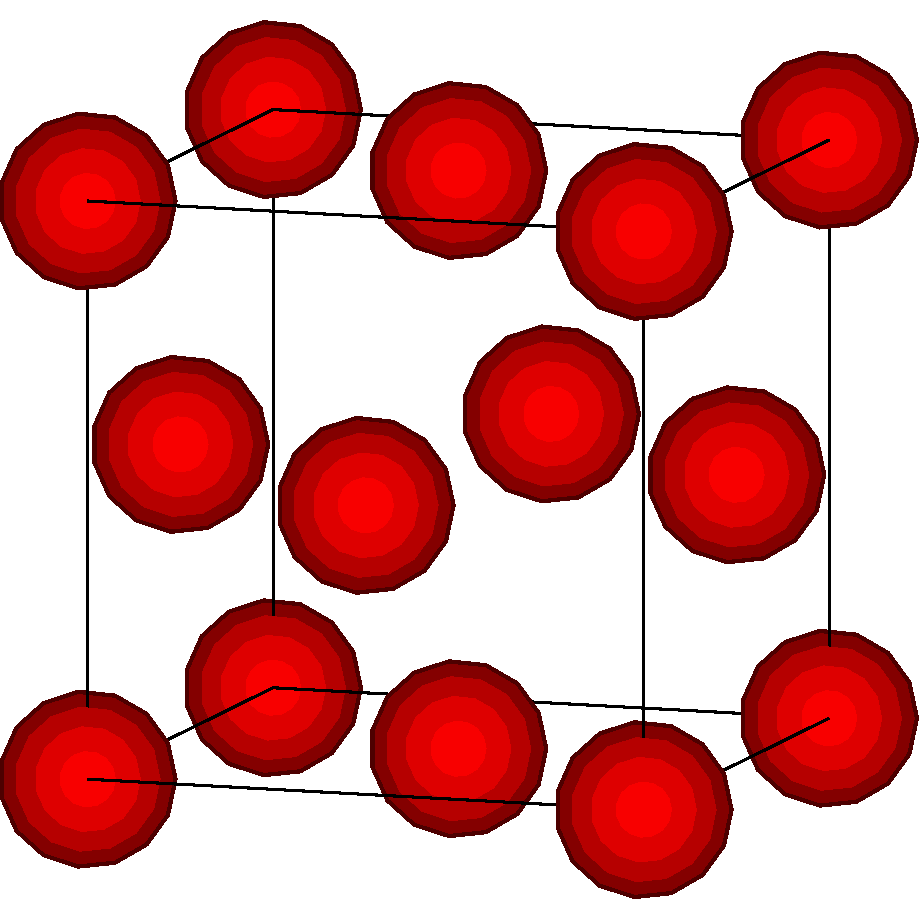
\includegraphics[width=\textwidth]{../assets/theorie/fcc}
        \caption{fcc-Gitter.} \label{fcc}
    \end{subfigure}
    \begin{subfigure}[t]{0.3\textwidth}
        \centering
        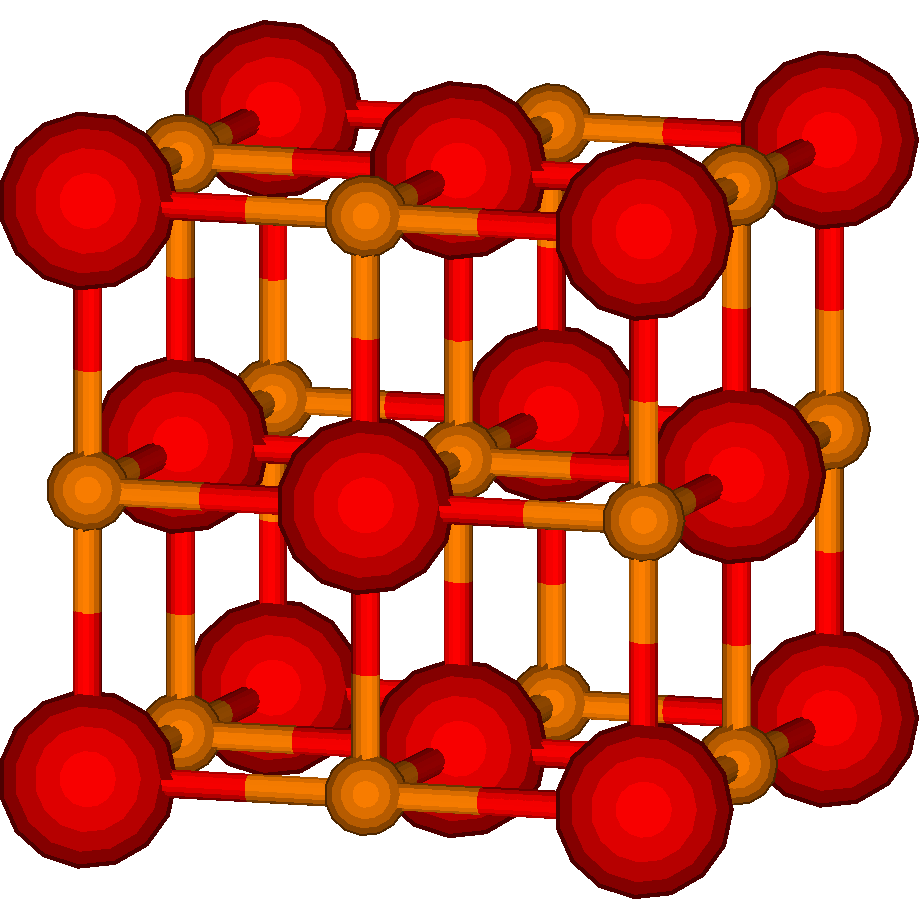
\includegraphics[width=\textwidth]{../assets/theorie/rocksalt}
        \caption{NaCl-Gitter} \label{nacl}
    \end{subfigure}
    \begin{subfigure}[t]{0.3\textwidth}
        \centering
        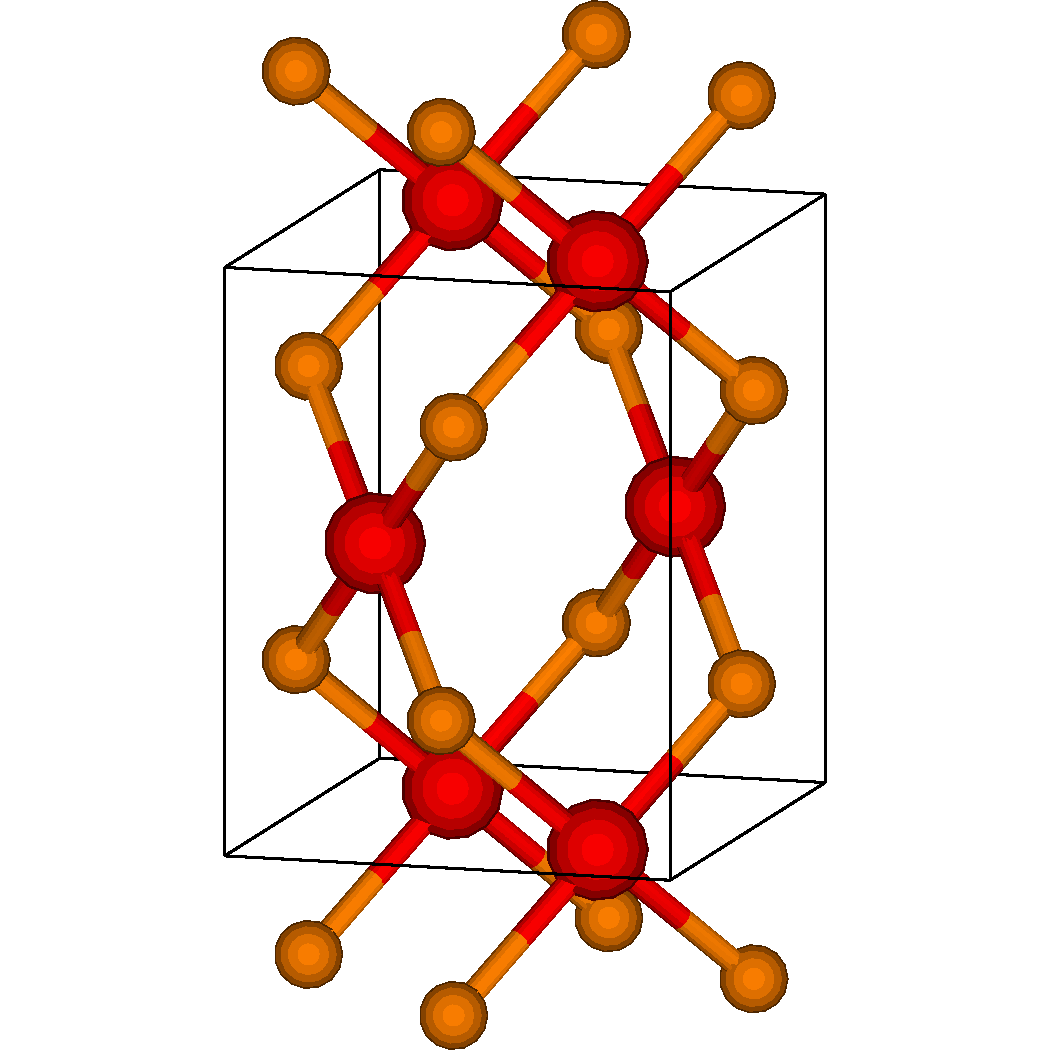
\includegraphics[width=\textwidth]{../assets/theorie/CuO}
        \caption{\ce{CuO}-Gitter} \label{cuo}
    \end{subfigure}
    \begin{subfigure}[t]{0.3\textwidth}
        \centering
        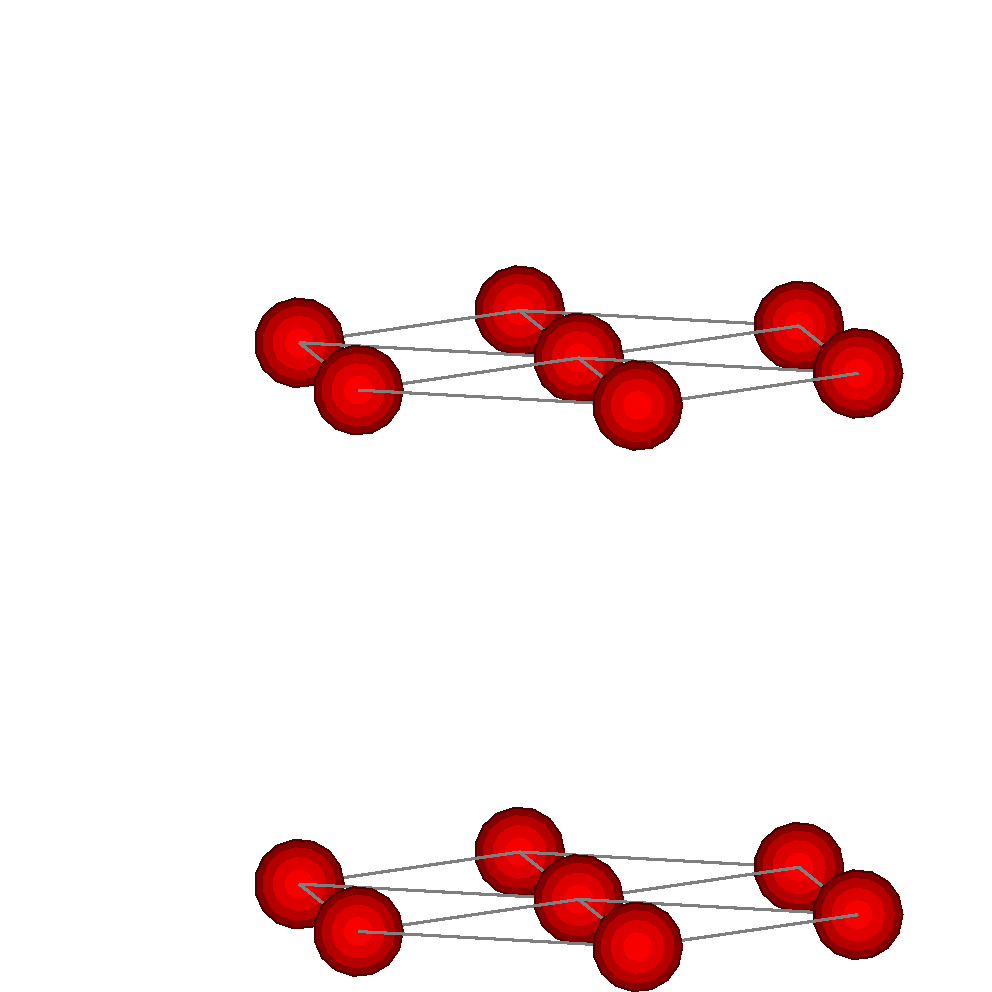
\includegraphics[width=\textwidth]{../assets/theorie/hex}
        \caption{hexagonales Gitter} \label{hex}
    \end{subfigure}
    \begin{subfigure}[t]{0.3\textwidth}
        \centering
        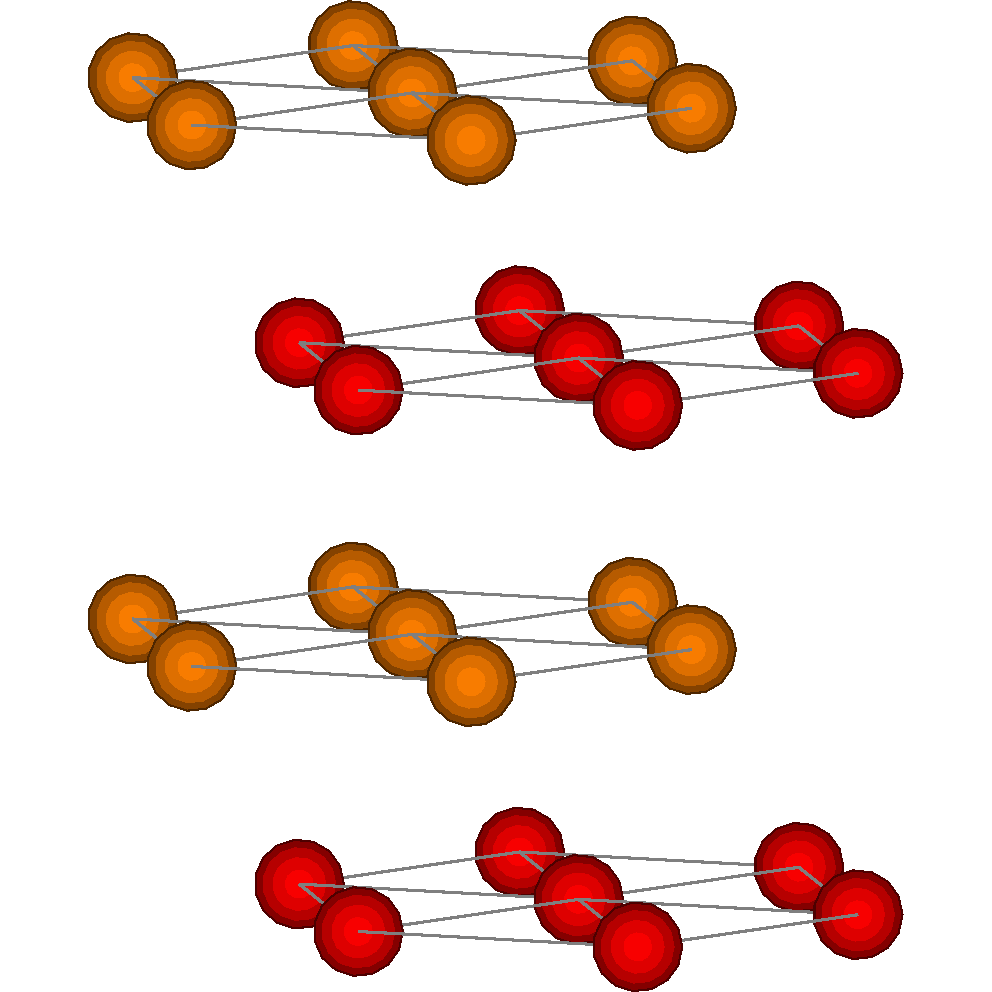
\includegraphics[width=\textwidth]{../assets/theorie/hcp}
        \caption{hcp-Gitter} \label{hcp}
    \end{subfigure}
    \begin{subfigure}[t]{0.3\textwidth}
        \centering
        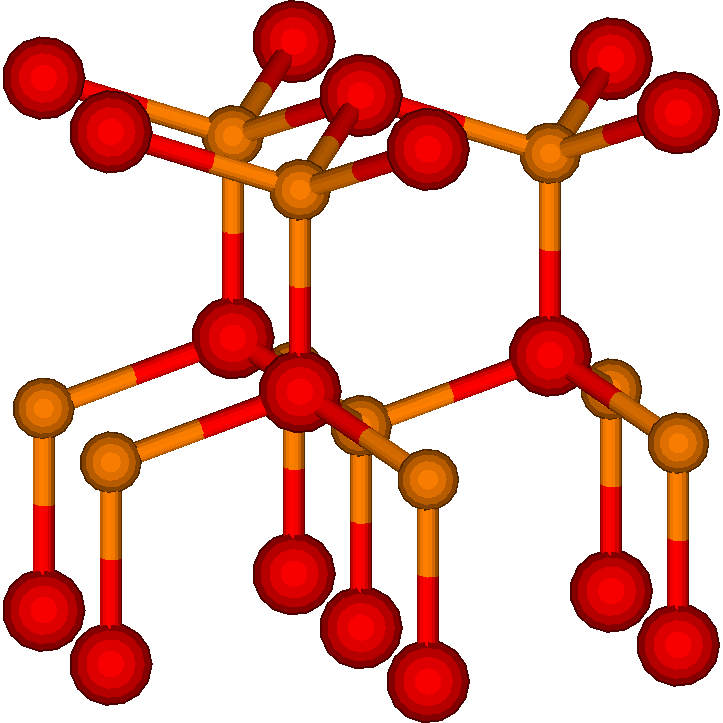
\includegraphics[width=\textwidth]{../assets/theorie/wurzite}
        \caption{Wurtzit-Gitter} \label{wurtzit}
    \end{subfigure}
    \caption{Ausgewählte Kristallgitter für die Untersuchung von \heo.} \label{fig:gitterstrukturen}
\end{figure}

\paragraph{Natriumchloridstruktur}
Die erste und wichtigste Kristallstruktur ist die Natriumchloridstruktur.
Um diese zu verstehen, betrachtet man zuerst ein kubisch-flächen\-zen\-trier\-tes Gitter (fcc, engl.
\textit{face-centered cubic}) welches durch die primitiven Vektoren
\begin{equation}
    \mathbf{a}_1 = a / 2 (\hat{x} + \hat{y}), \quad
    \mathbf{a}_2 = a / 2 (\hat{y} + \hat{z}), \quad
    \mathbf{a}_3 = a / 2 (\hat{x} + \hat{z})
    \label{eq:fcc}
\end{equation}
definiert ist.
Die Gitterpunkte liegen an Würfelecken und den dazugehörigen Flächenmittelpunkten, wie in \cref{fcc} dargestellt.
\autocite[37-38]{Grundmann}
Die Natriumchloridstruktur entsteht aus einem fcc-Gitter mit zweiatomiger Basis.
Dabei ist das erste Basisatom an der Gitterposition $(0,0,0)$ und das zweite an der Position $(a/2,a/2,a/2)$, wie in
\cref{nacl} dargestellt.\autocite[45]{Grundmann}
Sowohl Magnesiumoxid (\ce{MgO}), Kobaltoxid (\ce{CoO}) und Nickeloxid (\ce{NiO}) kristallisieren in dieser Struktur.
Auch \heo\ kristallisiert in der Natriumchloridstruktur, wenn
Sauerstoff als erstes Basisatom und ein zufällig ausgewähltes Metall als zweites Basisatom betrachtet wird.
\autocite[5]{Rost2015}

\paragraph{Tenoritstruktur}
Kupferoxid (\ce{CuO}) kristallisiert in einer monoklinen Kristall\-struk\-tur mit achtatomiger Basis.
Dabei sind vier dieser Basisatome Kupferatome und vier Sauerstoffatome.
Die Struktur ist in \cref{cuo} dargestellt.\autocite[7]{kupferoxid}

\paragraph{Wurtzitstruktur}
Um die Wurtzitstruktur zu verstehen, betrachtet man zuerst die einfach-hexagonale Struktur, die durch die primitiven
Vektoren
\begin{equation}
    \mathbf{a}_1 = a\hat{x}, \quad
    \mathbf{a}_2 = a/2 (\hat{x} + \sqrt{3} \hat{y}), \quad
    \mathbf{a}_3 = c \hat{z}
    \label{eq:hex}
\end{equation}
definiert ist.
Es entsteht ein Gitter, welches an den Ecken eines Sechsecks und den dazugehörigen Flächenmittelpunkten Gitterpunkte
besitzt, wie in \cref{hex} dargestellt.
Aus der einfach-hexagonalen Struktur ergibt sich die hexagonal dichtest gepackte Struktur
(hcp, engl. \textit{hexagonal-closed packet}).
Dieser liegt ein einfach-hexagonales Gitter mit zweiatomiger Basis bei den Gitterpositionen $(0,0,0)$ und
$(\mathbf{a}_1/3 + \mathbf{a}_2/3 + \mathbf{a}_3/2)$ zugrunde, wie in \cref{hcp} dargestellt.\autocite[97-98]{Ashcroft}
Die Wurtzitstruktur besteht aus einem einfach-hexagonalen Gitter mit vieratomiger Basis.
Eine bessere Vorstellung ergibt sich jedoch aus der Betrachtung zweier übereinander liegender hcp-Gitter, die um
die Höhe $\sqrt {3 / 8} a$ gegeneinander verschoben sind, wie in \cref{wurtzit} dargestellt.
Zinkoxid (\ce{ZnO}) kristallisiert in dieser Struktur.\autocite[47-48]{Grundmann}

\subsubsection{Reziprokes Gitter}
Das reziproke Gitter spielt für die weitere Betrachtung periodischer Strukturen eine fundamentale Rolle.
Ziel ist es, eine Funktion zu konstruieren, die gitterperiodisch im Bravaisgitter ist.
Für diese Funktion soll also gelten
$f(\mathbf{x})=f(\mathbf{x}+\mathbf{O})$, falls $\mathbf{O}=\sum_{i=1}^{3} \alpha_{i}\mathbf{a}_{i}$.
Mithilfe einer Reihenentwicklung ergibt sich die folgende, allgemeine Form:
\begin{align}
    \begin{split}
        f(\mathbf{x})&=\sum_{\mathbf{R}}a_{\mathbf{R}}\cdot \exp(\mathrm{i}\mathbf{R}\cdot\mathbf{x}),\\
        f(\mathbf{x}+\mathbf{O})&=\sum_{\mathbf{R}}a_{\mathbf{R}}\cdot \exp(\mathrm{i}\mathbf{R}\cdot \mathbf{x})\cdot
        \underbrace{ \exp(\mathrm{i}\mathbf{R}\cdot \mathbf{O}) }_{ \stackrel{!}{=}1 }  \stackrel{!}{=} f(\mathbf{x}).
    \end{split}
\end{align}
Erkennbar ist die notwendige Bedingung $\exp(\mathrm{i}\mathbf{R}\cdot \mathbf{O})=1$.
Dies ist äquivalent zur Aussage $\mathbf{R}\cdot \mathbf{O}=2\pi z$ mit $z \in \mathbb{Z}$.
Damit lässt sich das reziproke Gitter durch die Menge
$\{ \mathbf{R} \,\vert\, \exp(\mathrm{i}\mathbf{R}\cdot \mathbf{O})=1 \quad
\forall \mathbf{O} \in \text{span}(\mathbf{a}_{i}) \}$ definieren. \autocite[108]{Ashcroft}
Analog zum Ortsraum lassen sich auch hier primitiven Vektoren mit folgender Vorschrift bilden:
\begin{align*}
    \mathbf{b}_{1} = 2\pi \cdot \frac{\mathbf{a}_{2} \times \mathbf{a}_{3}}{V_{\mathrm{EZ}}} \quad
    \mathbf{b}_{2} = 2\pi \cdot \frac{\mathbf{a}_{3} \times \mathbf{a}_{1}}{V_{\mathrm{EZ}}} \quad
    \mathbf{b}_{3} = 2\pi \cdot \frac{\mathbf{a}_{1} \times \mathbf{a}_{2}}{V_{\mathrm{EZ}}}.
\end{align*}
Jeder Punkt im reziproken Gitter kann durch $\sum_{i=1}^{3} \beta_{i}\mathbf{b}_{i}$ mit $\beta_i \in \mathbb{Z},
i\in\{1,2,3\}$ beschrieben werden.
Es gilt die Relation $\mathbf{b}_{i}\cdot \mathbf{a}_{j}=2 \pi \delta_{ij}$.
Hierbei ist $\delta_{ij}$ das Kronecker-Delta.
\autocite[109]{Ashcroft}

\subsubsection{Indizierung von Gitterebenen und Gitterrichtungen}\label{subsubsec:indizierung}
Die erste wichtige Anwendung des reziproken Gitters ist die Charakterisierung von Gitterebenen.
Eine Gitterebene ist eine beliebige, im Bravaisgitter liegende Ebene, die mindestens drei nicht kollineare Gitterpunkte
enthält.
Aufgrund der Kristallsymmetrie liegen damit unendlich viele weitere Gitterpunkte innerhalb dieser Ebene.
Mithilfe der Translationssymmetrie findet man parallele Gitterebenen im Abstand $d$.
Diese fasst man als Gitterebenenscharen zusammen. \autocite[113]{Ashcroft}

Gitterebenenscharen kann man mithilfe des reziproken Gitters charakterisieren, denn für jede
Gitterebenenschar im Abstand $d$ existieren Vektoren des reziproken Gitters, welche senkrecht auf den Ebenen stehen.
Für die eindeutige Beschreibung wählt man den kleinsten dieser Vektoren $\mathbf{r}$, welche stets die Länge $2 \pi / d$ besitzt.
Auch die Umkehrung gilt: Für jeden Vektor $\mathbf{R}$ aus dem reziproken Gitter, existiert eine Schar von senkrechten
Gitterebenen.
Der Abstand $d$ dieser Ebenen ist an den Betrag des kleinsten parallelen Vektors $\mathbf{r}$ durch $\lvert \mathbf{r}
\rvert=2\pi  /d$ gekoppelt.
Es existiert also eine einfache Möglichkeit, Gitterebenen mithilfe von reziproken Gittervektoren eindeutig zu
identifizieren. \autocite[113]{Ashcroft}

Um Gitterebenenscharen zu kennzeichnen, verwendet man die Millerschen Indizes.
Sei dazu $\mathbf{r}$ der kürzeste reziproke Gittervektor, welcher senkrecht auf der zu charakterisierenden Ebene steht.
Dieser lässt sich darstellen durch $ \mathbf{r} = h \mathbf{b_1} + k \mathbf{b_2} + l \mathbf{b_3}$.
Das Tupel $(h\, k\,l)$ sind die Millerschen Indizes, welche definitionsgemäß aus ganzen Zahlen bestehen müssen.


Es existiert eine geometrische Interpretation, die es erlaubt, die Indizes im Ortsraum zu
visualisieren.
Für jede Gitterebene findet man ein entsprechendes $A$, sodass die Ebenengleichung $\mathbf{r} \cdot \mathbf{x} = A$
erfüllt ist.
Nun definiert man die Durchstoßpunkte zwischen den durch die primitiven Vektoren $\mathbf{a}_i$ aufgespannten
Koordinatenachsen und der Ebene durch die Zahlen $x_{1}\mathbf{a}_{1}, x_{2}\mathbf{a}_{2}, x_{3}\mathbf{a}_{3}$.
Da die Durchstoßpunkte in der Ebene liegen, ist die Ebenengleichung $\mathbf{r}\cdot(x_{i}\mathbf{a}_{i})=A$ erfüllt und
man findet mit $\mathbf{r}\cdot\mathbf{a}_{1}=2\pi h$, $\mathbf{r}\cdot \mathbf{a}_{2}=2\pi k$,
$ \mathbf{r}\cdot \mathbf{a}_{3}=2\pi l$ folgenden Zusammenhang:
\begin{equation*}
    x_{1}=\frac{A}{2\pi h}, \quad x_{2}=\frac{A}{2\pi k}, \quad x_{3} =\frac{A}{2\pi l}.
\end{equation*}
Kennt man die Achsendurchstoßpunkte $x_i$, kann man die Millerschen Indizes finden, indem man den Parameter $A$
kleinstmöglich wählt, sodass $h$, $k$ und $l$ ganzzahlig sind. \autocite[115]{Ashcroft}

Nicht nur Gitterebenen, sondern auch Gitterrichtungen lassen sich in ähnlicher Weise indizieren.
Das Tupel $[h\,k\,l]$ beschreibt diejenige Richtung, die durch den Vektor $\mathbf{O} = h\mathbf{a}_{1}+k\mathbf{a}_{2}+
l\mathbf{a}_{3}$ vorgegeben wird.
Zu beachten ist, dass Richtungsvektoren in unserem Kontext im Ortsraum leben,
währenddessen Ebenennormalenvektoren durch Vektoren im reziproken Raum dargestellt werden.
Um dies zu verdeutlichen werden eckige anstelle der runden Klammern verwendet.
Es existiert weiterhin eine besondere Notation zur Kennzeichnung äquivalenter Gitterebenenscharen und Raumrichtungen.
In diesem Kontext bedeutet das, dass die Möglichkeit besteht, äquivalente Gitterebenenscharen und Raumrichtung durch
Symmetrieoperationen ineinander zu überführen.
Äquivalente Ebenen notiert man mit $\{h \,k\, l \}$, für Richtungen gilt entsprechend $\langle h\, k \, l \rangle$.
\autocite[116]{Ashcroft}

\subsubsection{Röntgenbeugung und die Laue Bedingung}
Ziel ist es, mithilfe elektromagnetischer Strahlung und den bisherigen Überlegungen, Aussagen über die
Kristallstruktur eines Festkörpers zu gewinnen.
Genauer gesagt sucht man einen Formalismus, um die elastische Streuung von Licht am Kristallgitter zu beschreiben.
Für eine geeignete Wellenlänge der Photonen betrachtet man die typische zwischenatomare Entfernung von circa
\qty{1}{\angstrom}.
Aus der Optik ist bekannt, dass mindestens eine Wellenlänge gleicher Größenordnung genutzt werden
muss, um beide Punkte hinreichend genau aufzulösen.
Entsprechend muss die Photonenenergie in der Ordnung von
$\h f =\h \c / \lambda \simeq \qty{12.3}{\electronvolt}$ liegen.
Hierbei ist $f$ die Frequenz, $\lambda$ die Wellenlänge, $\h$ das Plancksche Wirkungsquantum und $\c$ die
Lichtgeschwindigkeit.
Solche Energien sind charakteristisch für Röntgenstrahlung. \autocite[120]{Ashcroft}

Laue und Bragg entwickelten zwei Formalismen, um elastischen Streuung elektromagnetischer Strahlung am Kristallgitter
zu beschreiben.
Im Folgenden wird der Laue-Formalismus erklärt und die Äquivalenz zur Bragg-Bedingung gezeigt.

\paragraph{Streuung an zwei Gitterpunkten}
\begin{figure}
    \centering
    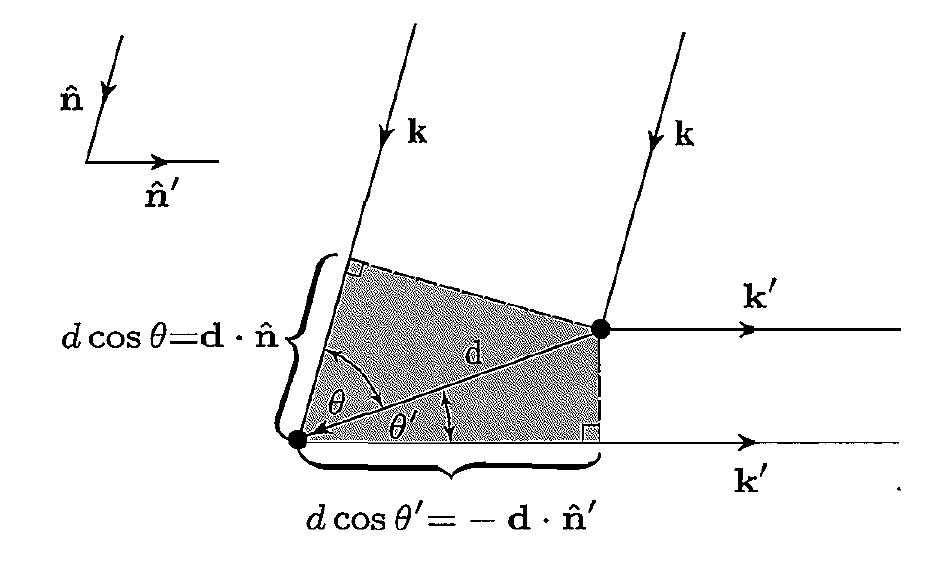
\includegraphics[width=0.5\textwidth]{../assets/theorie/lauebeugung}
    \caption{Skizze zur Erklärung der Laue-Bedingung. \imcitetwo[123]{Ashcroft}} \label{fig:laue}
\end{figure}
Zur Herleitung der Beugungsbedingung nach Laue betrachtet man die Bestrahlung zweier Gitterpunkte mit Photonen unter
Annahme von elastischen Streuung.
Der Abstand der Gitterpunkte ist durch den Vektor $\mathbf{O}$ gegeben.
Dabei ist die einfallende Strahlung durch den Wellenzahlvektor  $\mathbf{k}$ charakterisiert.
Es gilt der Zusammenhang $\lvert \mathbf{k} \rvert = 2 \pi / \lambda$ und die Dispersionsrelation
$\omega = \c \lvert \mathbf{k} \rvert$.
Die gestreute Strahlung wird durch den Wellenzahlvektor $\mathbf{k}'$ beschrieben.
Da nur elastische Streuung betrachtet wird, gilt $\lvert \mathbf{k} \rvert=\lvert \mathbf{k}' \rvert$.
Somit sind die Frequenzen ($\omega$ und $\omega'$) beider Wellen gleich.
Für den Wegunterschied $\Delta s$ findet man anhand \cref{fig:laue} den Zusammenhang:
\begin{equation}
    \Delta s = \Delta s_{1} + \Delta s_{2} = \underbrace{ \mathbf{O} \cdot \frac{\mathbf{k}}{\lvert \mathbf{k} \rvert }
    -\mathbf{O}\cdot \frac{\mathbf{k}'}{\lvert \mathbf{k}' \rvert}  }_{\substack{\text{Projektion von } \\ \mathbf{O} \text{ auf }
    \mathbf{k} \text{ bzw. }\mathbf{k'} }} =  \frac{\lambda}{2\pi} \mathbf{O}\cdot\Delta \mathbf{k}.
    \label{eq:laue}
\end{equation}
Hierbei ist $\Delta \mathbf{k} = \mathbf{k}-\mathbf{k}'$ der Differenzvektor der Wellenzahlvektoren.
Für konstruktive Interferenz muss die Bedingung $\Delta s = n \lambda, n \in \mathbb{N}$ erfüllt sein, sodass durch
Gleichsetzen die Beziehung $\mathbf{O}\cdot\Delta \mathbf{k} =2\pi n$ folgt.
Aus der geometrischen Anordnung der Gitterpunkte ergibt sich ein Wegunterschied, der äquivalent
zu einer Phasendifferenz von $\Delta\varphi=(2\pi / \lambda) \cdot \Delta s = \Delta \mathbf{k}\cdot \mathbf{O}$ ist.
\autocite[122-123]{Ashcroft}

Unter der Annahme, dass beide Gitterpunkte Kugelwellen mit Amplituden $u_{0}(\mathbf{r})$ und $u_{1}(\mathbf{r})$
ausstrahlen, ergibt sich für die Überlagerung beider Wellen die folgende Form:
\begin{align}
    u(\mathbf{r},t)=u_{0}(\mathbf{r})\cdot \exp(\mathrm{i}\omega t+\mathrm{i}\lvert \mathbf{k}
    \rvert r) + u_{1}(\mathbf{r}) \cdot \exp(\mathrm{i}\omega t + \mathrm{i}\lvert \mathbf{k}
    \rvert r+\mathrm{i}\Delta\varphi).
\end{align}
Die Überlagerung der beiden Wellen führt zu einer Interferenz, die durch die Phasendifferenz $\Delta\varphi$ bestimmt
wird.

\paragraph{Streuung an allen Gitterpunkten}
Will man die Streuung im gesamten Kristall betrachten, muss über alle Streuzentren, das heißt über alle Gittervektoren,
im Kristall summiert werden.
Diese sind gegeben durch $\mathbf{O}_{pqr}=p\mathbf{a}_{1}+q\mathbf{a}_{2}+r\mathbf{a}_{3}$.
Für die Superposition aller Wellen mit Amplitude $u_{pqr}(\mathbf{r})$ und Phasendifferenz $\Delta\varphi_{pqr}$
ergibt sich:
\begin{align}
    \begin{split}
        u(\mathbf{r}, t)
        &=\sum_{pqr} u_{pqr}(\mathbf{r})\cdot \exp(\mathrm{i}\omega t+\mathrm{i}
        \lvert \mathbf{k} \rvert r+\mathrm{i}\underbrace{ \Delta\varphi_{pqr} }_{ = \Delta
        \mathbf{k}\cdot \mathbf{O}_{pqr}})) \\
        &=\exp(\mathrm{i}\omega t+\mathrm{i}\lvert \mathbf{k} \rvert r)\cdot
        \underbrace{ \sum_{pqr}u_{pqr}(\mathbf{r})\cdot \exp(\mathrm{i}\Delta \mathbf{k}
        \cdot \mathbf{O}_{pqr}) }_{ \coloneqq A }.
    \end{split}
    \label{eq:amplitude}
\end{align}
Die Größe $A$ wird als Streuamplitude bezeichnet.
Die tatsächliche Streuung erfolgt an der Elektronenverteilung.
Das führt zu zusätzlichen Effekten wie dem Atomformfaktor und dem Strukturfaktor,
welche für weitere Betrachtungen jedoch vernachlässigt werden können:\autocite[66-69]{Spiess}
\begin{equation}
    A \propto \int n(\mathbf{r}) \exp(\mathrm{i} \Delta \mathbf{k}\cdot
    \mathbf{r}) \, \mathrm{d}V(\mathbf{r}).
    \label{eq:atomformfaktor}
\end{equation}

\paragraph{Beugungsbedingung}
Die Bedingung für konstruktive Interferenz ist äquivalent zur Maximierung der Streuamplitude.
Damit diese maximal wird, muss die Interferenzbedingung $\mathbf{O}_{pqr}\cdot\Delta \mathbf{k} =2\pi z$
für alle $p$, $q$, $r$ gelten.
Zerlegt man $\mathbf{O}_{pqr}$ in seine Komponenten, erhält man folgende Gleichungen:
\begin{equation}
    \mathbf{a}_{1}\cdot\Delta \mathbf{k} = 2\pi h, \quad
    \mathbf{a}_{2}\cdot\Delta \mathbf{k} = 2\pi k, \quad
    \mathbf{a}_{3}\cdot\Delta \mathbf{k} = 2\pi l
    \label{eq:lauebedingung}
\end{equation}
Dies sind die Laue Gleichungen für Beugungsmaxima.
Sie sind erfüllt, falls $\Delta \mathbf{k}$ ein reziproker Gittervektor ist.
Es stellt die Beugungsbedingung nach Laue dar, die besagt, dass konstruktive Interferenz genau dann auftritt,
wenn $\Delta \mathbf{k}$ einem Vektor des reziproken Gitters entspricht.\autocite[125]{Ashcroft}

Für die Strukturamplitude ergibt sich anschließend:
\begin{equation}
    A = \sum_{pqr} u_{pqr}(\mathbf{r}) \cdot\underbrace{ \exp(2\pi \mathrm{i}
    \cdot(\underbrace{ mh+nk+pl }_{ \in\mathbb{Z} })) }_{ =1 }
    = \sum_{pqr} u_{pqr}(\mathbf{r}).
    \label{eq:strukturamplitude}
\end{equation}

\paragraph{Bragg-Bedingung}
Die Bragg Bedingung kann sowohl mithilfe der Laue-Bedingung als auch geometrisch hergeleitet werden.
Um die Äquivalenz zur Laue-Bedingung zu zeigen, wird die Bragg-Bedingung im Folgenden aus der Laue-Bedingung
hergeleitet.
Betrachtet man die einen Differenzvektor $\Delta \mathbf{k}=\mathbf{k}'-\mathbf{k}$, wobei $\mathbf{k}$ und
$\mathbf{k'}$ den Winkel $\alpha$ einschließen,so ist sein Betrag gegeben durch:
\begin{align}
    \begin{split}
        \lvert \Delta \mathbf{k} \rvert ^{2}&=\langle \Delta \mathbf{k} ,\Delta \mathbf{k}\rangle =\langle
        \mathbf{k}-\mathbf{k}', \mathbf{k}-\mathbf{k}' \rangle = k^{2}+k'^{2}-2kk'\cos(\alpha)  \\
        &=2{k}^{2}(1-\cos(\alpha))=4k^{2}\sin ^{2}\left( \frac{\alpha}{2} \right)
    \end{split}
\end{align}
Hierbei ist $\nu = \alpha / 2$ der Bragg-Winkel und $\langle \cdot , \cdot \rangle$ das Standardskalarprodukt.
Da $\Delta \mathbf{k}$ ein Vektor aus dem reziproken Raum ist und senkrecht auf der Gitterebene
steht, an welcher er gestreut wird, existiert ein kürzester Vektor $\mathbf{g}$, sodass
$n\cdot \mathbf{g} =\Delta \mathbf{k}$.
Aus \cref{subsubsec:indizierung} ist bekannt, dass $\mathbf{g}$ den Abstand der Netzebenen definiert
mit $d = 2 \pi \cdot\lvert \mathbf{g} \rvert ^{-1}$.
Daraus folgt $\lvert \Delta \mathbf{k} \rvert=n \lvert \mathbf{g} \rvert = 2\pi n/d$.
Kombiniert man beide Gleichungen miteinander, ergibt sich die Bragg-Bedingung:\autocite[125-126]{Ashcroft}
\begin{align}
    \begin{split}
        2k\sin(\nu)&=\frac{2\pi n}{d} \\
        2d\sin(\nu)&=n \lambda
    \end{split}
\end{align}

\subsection{Entropiestabilisierte Metalloxide}\label{subsec:hochentropische-metalloxide}
Die Suche nach neuen fortschrittlichen Materialien, welche die Bedürfnisse moderner Technologien erfüllen, ist ein
wichtiger Bestandteil der Materialwissenschaften.
Ein vielversprechender alternativer Ansatz, der sich in den letzten Jahren etablierte, ist die Herstellung und
Untersuchung hochentropischer Materialien.
Bereits Cantor et al.\ untersuchte 2004 die Eigenschaften von Mehrkomponentenlegierungen, bestehend aus 20,
beziehungsweise 16 equimolar verteilten Elementen.
Beide Systeme zeigten mehrere Phasen, aber auch eine gemeinsame fcc Struktur.
Mithilfe dieser Beobachtung konnte Cantor das Fünf-Komponenten-System \ce{CrMnFeCoNi} entwickeln, welches in einphasiger
fcc-Struktur kristallisiert und schaffte damit den Grundstein für
die Entwicklung mehrkomponentiger Legierungen.\autocite{cantor}

Yeh et al.\ konnten das Phänomen mithilfe der Mischungsentropie erklären und führten den Begriff der
hochentropischen Legierungen (HEAs, engl. \textit{high entropy alloys}) ein.
Dabei klassifizierten sie Legierungen als HEAs, falls diese mindestens fünf oder mehr Komponenten besitzen
und das molare Verhältnis jedes Konstituenten zwischen \qty{5}{\percent} und \qty{35}{\percent} liegt.\autocite{yeh}

Rost et al.\ erweiterten 2015 das Konzept der HEAs auf Metalloxide und führten den Begriff der hochentropischen
Metalloxide (HEOs, engl. \textit{high entropy oxides}) ein.
Sie synthetisierte das Material \heo\ und untersuchten dessen Struktur und Eigenschaften.
Dabei fand sie heraus, dass \heo\ in einer einzigen Phase kristallisiert und
schuf damit die Grundlage für ein neues Forschungsfeld in der Materialwissenschaft.\autocite{Rost2015}

\subsubsection{Struktur von \heo}
\begin{figure}
    \centering
    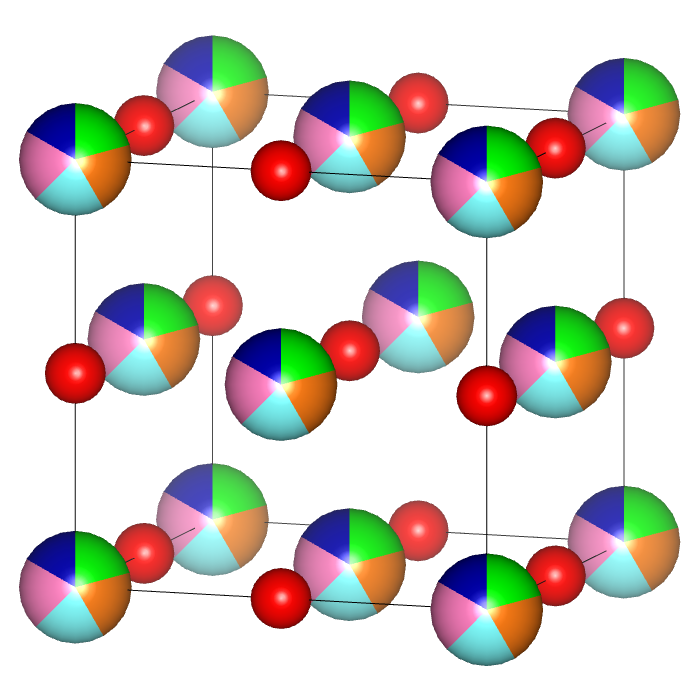
\includegraphics[width=0.3\textwidth]{../assets/theorie/heo}
    \caption{Struktur von \heo. Rot: Sauerstoff, Bunt: Metallkationen.}
    \label{fig:heo}
\end{figure}
In Analogie zu den HEAs ist \heo\ ein Mehrkomponentenoxid, welches in einer Natriumchloridstruktur kristallisiert.
Die Kationenstelle ist durch ein zufälliges Metallkationen \ce{Mg^{2+}}, \ce{Co^{2+}}, \ce{Ni^{2+}},
\ce{Cu^{2+}} oder \ce{Zn^{2+}} besetzt.
Im Kontrast zu den HEAs existiert ein geordnetes Anionengitter, welches durch Sauerstoffionen besetzt ist.
Die Struktur von \heo\ ist in \cref{fig:heo} dargestellt.\autocite[5]{Rost2015}
Es ist bemerkenswert, dass diese Phase stabil synthetisiert werden konnte, insbesondere angesichts der Änderungen in der
Kristallstruktur von \ce{ZnO} und \ce{CuO} sowie der damit verbundenen Energie.
Um dieses Phänomen zu verstehen, muss die Rolle der Gibbs-Energie und der darin auftretenden Entropie
erläutert werden.

\subsubsection{Gibbs-Energie und Phasenstabilität}
Aus der Thermodynamik ist bekannt, dass ein Prozess genau dann freiwillig abläuft, falls die Gesamtentropie des
Systems und seiner Umgebung zunimmt.
Beschränkt man sich auf Prozesse, die bei konstantem Druck und Temperatur ablaufen, dann ist diese Aussage äquivalent
zur Minimierung der Gibbs-Energie $G$.
In der einfachsten Betrachtung ist diese folgendermaßen definiert:
\begin{align}
    \begin{split}
        G(T,p, \{ n_{i} \})&=H(T,p,\{ n_{i} \})-TS(T,p,\{ n_{i} \}), \\
        \Delta G(T, p, \{ n_{i} \})&=\Delta H(T,p, \{ n_{i} \})-T \Delta S(T,p, \{ n_{i} \})
    \end{split}
    \label{eq:gibbs}
\end{align}
Hierbei ist $H$ die Enthalpie, $S$ die Entropie, $T$ die Temperatur, $p$ der Druck und $n_{i}$ die Stoffmengen jener
Komponenten, die am Prozess beteiligt sind.
Das $\Delta$ symbolisiert die Änderung der jeweiligen Größe.
Die Gibbs-Energie ist eine Zustandsgröße und hängt nur von den Größen $T$, $p$ und $\{ n_{i} \}$ ab.
Die Änderung der Gibbs Energie $\Delta G$ ist ein Maß für die Spontanität eines Prozesses.
Ist $\Delta G < 0$, so läuft der Prozess freiwillig in einen energetisch günstigeren Zustand ab.
Aus dieser Forderung ist ersichtlich, dass der stabilste Zustand die Gibbs-Energie minimiert.\autocite[7]{rost_phd}


Die Gibbs-Energie ist maßgeblich von Enthalpie, Temperatur und Entropie abhängig.
Für vergleichsweise niedrige Temperaturen ist die Enthalpie der dominierende Faktor.
Nicht selten sind Enthalpie-minimierte Zustände diejenigen, die auch die Gibbs-Energie minimieren.
Für hochentropische Materialien ist das in der Regel nicht der Fall.
Diese zeichnen sich dadurch aus, dass sie eine hohe Entropie besitzen, sodass das System
bei entsprechend hohen Temperaturen in einen anderen, als den Enthalpie-minimalen Zustand übergeht.
Dieser Zustand ist dann durch die Entropie stabilisiert.\autocite[2]{Rost2015}

\subsubsection{Mischungsentropie}
Nun stellt sich die Frage nach der genauen Form der Entropie, die die Phasenstabilität von \heo\ beeinflusst.
Für diese Beschreibung zieht man das Modell der idealen Lösung heran.
Dies ist eine Mischung aus zwei oder mehreren Komponenten, deren Entstehung nicht mit einer Änderung der
Wärme oder Volumenänderung verbunden ist.
Dabei wird die Entropie der Mischung mithilfe der Mischungsentropie von Idealgasen beschrieben.
Für diese findet man die folgende Form:
\begin{equation}
    \Delta S_{\text{Misch}} = -\mathrm{R} \sum_{i=1}^N x_{i} \ln(x_{i}).
    \label{eq:Mischungsentropie}
\end{equation}
Hierbei ist $\mathrm{R}$ die allgemeine Gaskonstante, $x_{i}$ die Stoffmengenanteile der Komponenten und $N$ die Anzahl
der Komponenten.
Das Maximum der Entropie wird erreicht, wenn alle Komponenten gleichmäßig verteilt sind.
Dann gilt $x_{i}=1/N$ und $\max(S_{\text{Misch}}) = \mathrm{R} \ln(N)$.\autocite[7]{rost_phd}

Eine weitere Möglichkeit zur Visualisierung der Mischungsentropie ergibt sich, indem man die Konzentration eines
Konstituenten variiert und alle anderen konstant hält.
Mit der Parametrisierung $x_{1} = x$ und $x_{j} = (1-x) / (N-1)$ für $j=2, \dots, N$ ergibt sich für die
Mischungsentropie:

\begin{equation}
    \Delta S_{\text{Misch}} = -R \left( x \ln(x) + (1-x) \ln \left( \frac{1-x}{N-1} \right) \right).
    \label{eq:Mischungsentropie2}
\end{equation}

\begin{figure}
    \centering
    \import{../plots/theory}{mixing_entropy.pgf}
    \caption{Darstellung der Mischungsentropie in Abhängigkeit der Konzentration bei $N$ Komponenten und Variation einer
    Komponente unter equimolarer Verteilung der übrigen Komponenten.
    \imcitetwo[3]{Rost2015}}
    \label{fig:Mischungsentropie}
\end{figure}

Diese ist in \cref{fig:Mischungsentropie} dargestellt.
Hieraus ist erneut erkennbar, dass die Mischungsentropie maximal wird, wenn alle Komponenten gleichmäßig verteilt sind.
\autocite[3]{Rost2015}

Im Bezug auf die Gibbs-Energie impliziert dies, das die für den Phasenübergang nötige Temperatur umso niedriger sein
kann, je höher die Mischungsentropie ist.
Für eine äquimolare Verteilung ist die geringste Temperatur notwendig, um den Phasenübergang zu erreichen.

\subsubsection{Ideale und reale Lösungen}
Mithilfe der idealen Lösung konnte die Mischungsentropie von \heo\ beschrieben werden.
Problem ist, dass in diesem Modell die Enthalpie der Mischung nicht verändert wird.
Für die ideale Lösung gilt $\Delta H_\mathrm{Misch} = 0$.
In der Realität ändern sich jedoch Bindungsenergien der Atome.
Wie in \cref{subsubsec:kristallgitter} erläutert, kristallisiert $\ce{CuO}$ in der Tenoritstruktur, $\ce{ZnO}$ in der
Wurtzitstruktur wohingegen \heo\ in der Natriumchloridstruktur kristallisiert.
Auch die übrigen Konstituenden ändern ihre Gitterkonstanten leicht.
Die Änderungen solcher Bindungsenergien ändern die Enthalpie der Mischung und damit auch die Gibbs-Energie.
Um eine Erweiterung zu finden, die auch die Enthalpie der Mischung berücksichtigt, betrachtet man ein
Zweikomponentensystem, welches gemischt wird:
\begin{equation}
    \mathrm{A} + \mathrm{B} \longrightarrow \mathrm{AB}.
    \label{eq:reaktion}
\end{equation}
Die Mischungsentropie ist nach vorherigem Abschnitt gegeben durch:
\begin{equation}
    \Delta S_{\mathrm{mix}}=-R[x_{\mathrm{A}}\ln(x_{\mathrm{A}})+x_{\mathrm{B}}\ln(x_{\mathrm{B}})].
    \label{eq:Mischungsentropie3}
\end{equation}
Im einfachsten Modell einer realen Lösung besitzt die Mischungsenthalpie die einfache Form:
\begin{equation}
    \Delta H_{\mathrm{Misch}}= a x_{\mathrm{A}} x_{\mathrm{B}}.
    \label{eq:Mischungsenthalpie}
\end{equation}
Hierbei ist $a$ eine Konstante, die die Bindungsenergie der Mischung beschreibt.
Unter dieser Annahme wird die Enthalpie eine Kompositionsfunktion.
Je nach Vorzeichen von $a$ können entweder gleichatomige Bindungen ($a > 0$) oder ungleichatomige Bindungen
($a < 0$) enthalpisch bevorzugt sein.
In den meisten Fällen ist $a > 0$, da energetisch ungünstigere Bindungen durch die Mischung entstehen.
Der Sonderfall $a=0$ entspricht der idealen Lösung.
Somit kann eine Erweiterung der Änderung der Gibbs-Energie gefunden werden:

\begin{equation}
    \Delta G_{\mathrm{Misch}}=\Delta H_{\mathrm{Misch}}-T\Delta S_{\mathrm{Misch}}=a x_{\mathrm{A}} x_{\mathrm{B}}
    +RT[x_{\mathrm{A}}\ln(x_{\mathrm{A}})+x_{\mathrm{B}}\ln(x_{\mathrm{B}})]
    \label{eq:mischgibbs}
\end{equation}

\begin{figure}
    \centering
    \import{../plots/theory}{mixing_properties.pgf}
    \caption{Darstellung von Mischungsenthalpie, Mischungsentropie und Gibbs Energie der Mischung.
    \imcitetwo[10]{rost_phd}}
    \label{fig:mixing_properties}
\end{figure}

Diese Änderung, zusammen mit Enthalpie- und Entropieänderung, ist in \cref{fig:mixing_properties} dargestellt.
Es ist zu erkennen, dass für niedrige Temperaturen die Gibbs-Energie durch die Enthalpie dominiert wird.
Das Minima bei $x=0$ beziehungsweise $x=1$ weißt darauf hin, dass die Gibbs-Energie minimal ist, wenn die
Komponenten rein sind.
Erst mit steigender Temperatur beginnt die Mischungsentropie zu dominieren.
Dies sorgt für eine stabile Mischphase bei hohen Temperaturen, sodass das Minimum der Gibbs-Energie bei $x=0.5$ liegt.
\autocite[7-9]{rost_phd}

    \section{Probenherstellung und Messmethoden}\label{sec:messmethoden}
\subsection{Pulsed Laser Deposition}\label{subsec:pld}
Die erste Aufgabe des Versuchs besteht darin, \heo-Dünnfilme herzustellen, die eine Dicke von wenigen hundert
Nanometern aufweisen.
Um das zu erreichen, verwendet man Pulsed Laser Deposition (PLD).
Dafür wird ein Laserstrahl auf einen Festkörper, dem Target, ausgerichtet, welches beginnt zu
verdampfen und sich auf ein Substrat absetzt.
Im Folgenden soll dieser Mechanismus genauer beschrieben werden.

\subsubsection{Aufbau}
Ein PLD-System besteht aus einem Laser, einer Vakuumkammer und den darin befindlichen Komponenten.
\paragraph{Laser}
Der Laser (Light Amplification by Stimulated Emission of Radiation) bildet das Herzstück des gesamten PLD Prozesses.
In diesem wechselwirken Gasatome mit einem elektrischen Feld, sodass sie in einen angeregten Zustand übergehen.
Anschließend wird das Prinzip der stimulierten Emission genutzt.
Das angeregte Elektron verweilt vergleichsweise lange im angeregten Zustand und relaxiert durch ein
weiteres Photon von außerhalb zurück in den Grundzustand.
Bemerkenswerterweise haben beide Photonen dadurch identische Eigenschaften wie Phase, Amplitude und Frequenz.
Somit wird ein Lichtstrahl erzeugt, der sich durch Kohärenz und Monochromatizität auszeichnet.
Durch einen Satz von Spiegeln im Inneren des Lasers kann der Strahl durch die Stimulierung weiterer Gasatome
verstärkt werden.
Abschließend wird der Strahl durch ein halbdurchlässiges Fenster emittiert. \autocite[2296-2297]{pld}
\paragraph{Vakuumkammer}
Der Laserstrahl wird anschließend durch ein Fenster in die Vakuumkammer, dem nächsten Bestandteil des PLD Prozesses,
geleitet.
In dieser kann mithilfe von Vor- und Turbomolekularpumpen ein Vakuum in der Größenordnung von
\qty{e-4}{\milli\bar} erzeugt werden.
Zusätzlich können auch Hintergrundgase wie Sauerstoff, Stickstoff oder Argon in die Kammer eingelassen werden.
Das Vakuumlevel beeinflusst einerseits die Zusammensetzung der Plasmawolke, andererseits auch die
Zeit, die benötigt wird, um eine einzelne Schicht von Adsorbaten auf dem Substrat abzuscheiden.
Eine Reduktion des Drucks führt damit zu einer stabileren Umgebung für die Dünnfilmabscheidung.\autocite[2297-2298]{pld}
\paragraph{Targethalter, Substrathalter, Heizer}
In der Vakuumkammer ist ein scheibenförmiges Target an einer Halterung montiert, welches aus dem Material besteht, aus
dem der Dünnfilm hergestellt werden soll.
Da das Target durch den Laserstrahl nur an einer kleinen Stelle erhitzt wird, ist es notwendig,
dass sich das Target relativ zum Laserstrahl bewegt, um eine gleichmäßige Abtragung zu gewährleisten.
Dafür reicht eine einfache Rotation aus.

Hinzu kommt ein Substrathalter, auf dem das Substrat montiert wird.
Dieses kann durch einen Widerstandsheizer auf eine Temperatur von bis zu \qty{1000}{\celsius} beziehungsweise
mithilfe eines Laserheizers auf circa \qty{1500}{\celsius} erhitzt werden.
Das Substrat selbst hat üblicherweise die Maße von circa \qty{10}{\milli\meter\squared}.\autocite[2299]{pld}

\subsubsection{Abscheidungsprozess}
Mithilfe der oben genannten Komponenten kann der Abscheidungsprozess durchgeführt werden.
Die Laserphotonen treffen auf das Target und regen dort Elektronen an.
Diese erfahren einen Intraband-Übergang, wodurch sie in einen angeregten Zustand übergehen.
Durch die Elektron-Phonon-Wechselwirkung relaxiert das Elektron und gibt dabei Energie in Form von Phononen ab.
Dies führt zur Erhitzung des Targets, welche nicht nur an der Oberfläche, sondern auch im Inneren stattfindet.
Durch die hohe Temperatur beginnt das Target zu Verdampfen.

Auch die verdampften Konstituenten des Targets wechselwirken mit den Laserphotonen.
Durch Photoionisation werden Elektronen herausgelöst, sodass eine Plasmawolke entsteht.
Diese breitet sich in der Vakuumkammer in Richtung Substrat aus und beginnt sich auf dem diesem abzusetzen.
Durch Adsorptionsprozesse beginnt die Bildung eines Dünnfilms.\autocite[2299-2301]{pld}


\subsection{XRD}\label{subsec:xrd}
Nachdem die Dünnfilme hergestellt wurden, ist der nächste Schritt, ihre Struktur zu charakterisieren.
Zwischen Dünnfilmen und ihren korrespondierenden Massivkörpern existieren signifikante Unterschiede.
Diese resultieren vorrangig aus dem Verhältnis von Oberfläche zu Volumen, sowie den jeweiligen
Wachstumsbedingungen, wie Temperatur, Druck und Substrat.
Sie zeigen sich beispielsweise in der Qualität der Kristallinität, sowie in Kompositionsgradienten.
Da Proben mit unterschiedlichen Wachstumsbedingungen hergestellt wurden und deren Eigenschaften dadurch
maßgeblich beeinflusst werden, ist es notwendig, die Kristallinität der Dünnfilme zu charakterisieren.
Röntgendiffraktometrie (XRD, engl. \textit{X-Ray diffraction}) ist eine weit verbreitete Methode, um die
Kristallstruktur von Dünnfilmen zu bestimmen.
Dabei wird ein Röntgendiffraktometer verwendet.

\subsubsection{Röntgendiffraktometer}
Das Röntgendiffraktometer besteht aus fünf Hauptkomponenten: Röntgenquelle und Detektor, Ein- und Ausfallsoptik,
sowie dem Goniometer.
Zusätzlich ist das Diffraktometer durch eine Strahlungsschutzverkleidung abgeschirmt und mit einer Steuerungssoftware
verbunden.
Im Folgenden werden die einzelnen Komponenten näher erläutert.

\paragraph{Röntgenquelle}
Die Röntgenstrahlen werden in einer Röntgenröhre erzeugt.
In dieser werden Elektronen aus einer Wolfram-Glühkathode emittiert und durch das elektrische Feld auf eine Anode
beschleunigt.
Die Anode besteht meist aus hochreinem Kupfer.
Stromstärke und Beschleunigungsspannung der Röntgenröhre müssen so gewählt werden, dass die Energie beim Auftreffen der
Elektronen auf die Anode ausreicht, um die gebundenen Elektronen der Atome auf das nächsthöhere Energieniveau anzuregen.
Aufgrund der daraus resultierende Wärme muss die Anode ständig wassergekühlt werden.
Im hauseigenen Röntgendiffraktometer wird eine Beschleunigungsspannung von \qty{40}{\kilo\volt} und eine Stromstärke
von \qty{40}{\milli\ampere} verwendet.

Nach der Kollision zwischen Kupferatom und Elektron relaxiert das Elektron unter Bildung eines Röntgenphotons.
Man erhält ein Spektrum, welches durch die charakteristische Strahlung der Anode sowie durch Bremsstrahlung
geprägt ist.
Die charakteristische Strahlung wird vorrangig durch die K-Linien, insbesondere $K_{\alpha_1}$, $K_{\alpha_2}$
und K$_{\beta}$, dominiert.
Da $K_{\alpha_1}$ und $K_{\alpha_2}$ energetisch sehr nahe beieinander liegen, können sie nicht immer einzeln
aufgelöst werden.
Die $K_{\beta}$ Strahlung ist größtenteils unerwünscht und kann durch geeignete Filter unterdrückt werden.


Die Wolfram-Glühkathode emittiert unerwüschterweise nicht nur Elektronen, sondern auch Wolfram-Atome in kleinen Mengen.
Über längere Zeiträume führt dies zu einer nicht mehr zu vernachlässigenden Kontamination der Anode.
Dadurch können bei Elektronenstößen auch Wolfram-Atome angeregt werden, was zu einer zusätzlichen Wellenlänge im
Spektrum führt
In den späteren Messergebnissen sind diese Beiträge erkennbar.
Abschließend gelangen die Röntgenstrahlen durch ein Berylliumfenster in die Einfallsoptik.

\paragraph{Röntgendetektor}
Die durch die Röntgenquelle erzeugten Strahlen gelangen nach Reflektion an der Probe in den Detektor.
Dieser dient dazu, den reflektierten Strahl in ein elektrisches Signal umzuwandeln.
Kategorisieren kann man Röntgendektektoren nach ihrer Funktionsweise.
Eine weitere Unterteilung erfolgt nach der Dimensionalität des Detektors.
Es können Punktdetektoren (0D), Linien- (1D) oder Flächendetektoren (2D) verwendet werden.
Im hauseigenen Röntgendiffraktometer ist ein Halbleiterdetektor verbaut, der in verschiedenen Dimensionalitäten
arbeiten kann.
Wichtig ist, dass die maximale Zählrate des Detektors nicht überschritten wird.
Das führt zu nichtlinearen Antworten und kann den Sensor beschädigen.
Um das zu vermeiden, können Filter und Attenuatoren verwendet werden.

\paragraph{Goniometer}
Das Goniometer ist die mechanische Komponente des Röntgendiffraktometers.
Es besteht aus mehreren Drehachsen, die es ermöglichen, die Probe in unterschiedlichsten Winkeln auszurichten.
Nach der Braggschen Beugungstheorie ergeben sich konstruktive Interferenzen an denjenigen Winkeln, die der
Bragg-Bedingung genügen.
Existieren Möglichkeit, die Winkel für Quelle und Detektor zu variieren, kann diese Interferenz beobachtet werden.
Im Allgemeinen ist die Röntgenquelle jedoch fest, eine äquivalente Drehung von Probe und Detektor ist deshalb gängig.
In der einfachsten Betrachtungsweise muss das Goniometer also den Winkel zwischen Probe und Quelle ($\omega$) und dem
Winkel zwischen Probe und Detektor ($2\theta$) einstellen können.
Diese Freiheit reicht zwar für Pulverproben, jedoch nicht für Dünnfilme.
Zwar kann man mit beiden Freiheitsgraden Messungen durchführen, welche die out-of-plane Orientierung charakterisieren,
jedoch ist es nicht möglich, die in-plane Orientierung zu bestimmen.
Dafür werden weitere Achsen, wie $\varphi$ und $\chi$, benötigt.
Eine Konstruktion mit den vier Achsen wird Euler-Wiege genannt.
%%TODO



\subsection{AFM}\label{subsec:afm}
Das Raster-Kraft-Mikroskop ist ein hochpräzises Messinstrument zum Erfassen von Oberflächenstrukturen.
Anders als bei Licht- oder Elektronenmikroskopie wird hierbei eine mechanische Funktionsweise umgesetzt.
Dabei fährt eine Messapparatur, der Cantilever, rasterweise über eine Oberfläche und tastet diese ab.
Die auf den Cantilever wirkenden atomaren oder magnetischen Kräfte werden gemessen, woraus eine Topographiekarte der
Oberfläche erstellt wird.

\subsubsection{Schematischer Aufbau und Funktionsweise}
Die grundlegende Funktionsweise ist in Abbildung 1 dargestellt.
Markierung 1 zeigt den Cantilever, der mit einer Messspitze mit Dimensionen im Nanometerbereich ausgestattet ist.
Fährt diese über die Probe, siehe Markierung 2, so wirken Kräfte auf die Spitze, welche den Cantilever auslenken.
Diese Auslenkung wird mittels eines Ablenkungserkennungssystems, Markierung 3, ausgewertet.
Hierbei wird ein Laserstrahl an der Rückseite des Cantilevers reflektiert, welcher anschließend auf einen Photodetektor
trifft.
Dieser Detektor kann nun anhand der Intensitätsverteilung auf den einzelnen Sektoren die Auslenkung und Torsion des
Cantilevers messen.
Die gemessene Auslenkung wird an das Feedback System übergeben, was Markierung 4 zeigt.
Basierend auf dem gewählten Betriebsmodus wird versucht, die gemessene Kraft oder Amplitude konstant zu halten.
Mithilfe dieser Regulation wird ein Korrektursignal ausgegeben, welches die Position des Cantilevers anpasst.
Dies geschieht mithilfe von Piezoelementen, wodurch der Cantilever in x, y oder z-Richtung bewegt werden kann.
Die z-Position des Cantilevers wird aufgezeichnet und als Topographiesignal am Computer ausgewertet, siehe Markierung 5.
\subsubsection{PID System}
Damit eine möglichst genaue Topografiekarte aufgezeichnet werden kann, ist ein schnelles und präzises Regelsystem von großer Bedeutung.
Daraus resultiert ein Fehlersignal $\Delta S(t) = S(t)-S_0$, welches auf folgende Weise ausgewertet wird:
\begin{align*}
    \Delta S_{reg}(t) = \underbrace{ K_p * \Delta S(t) }_{\text{Proportional (1)}} + \underbrace{K_i * \integral{0}{t}{\Delta S(\tau)}{\tau}}_{\text{Integral (2)}}
    + \underbrace{K_d * \derivative{t}{\Delta S(t)}}_{\text{Differential (3)}}
\end{align*}

\textbf{1. Proportional:}
Das Ausgabesignal wird Proportional zum Eingabesignal mit Proportionalitätskonstante $K_p$ ausgegeben.
Dies ist die einfachste Art der Regulation, welche nur auf den aktuellen Zustand reagiert.
Der P-Regler zeichnet sich durch ein typisches Einschwingsignal aus, welches durch die Trägheit des Systems zustande kommt.
Durch die Phasendifferenz zwischen Eingangssignal und Ausgangsreaktion des Systems entsteht oft eine Überreaktion,
Diese Überschreitung ruft eine Gegenreaktion hervor, welche sich rekursiv zu einer Schwingung entwickelt.
Da schwache Eingabesignale auch nur schwache Ausgangssignale erzeugen, kann es bei dem P-Regler auch zu einem permanenten Offset zwischen
Ist- und Sollwert kommen.

\textbf{2. Integral:}
Um dieses Problem zu lösen, wird ein I-Regler verbaut.
Hierbei wird das Ausgangssignal proportional zum Integral des Eingabesignals mit Proportionalitätskonstante $K_i$ ausgegeben.

\textbf{3. Differential:}
Um die Güte des Reglers weiter zu verbessern, werden D-Regler verwendet.
Dabei wird das Ausgangssignal proportional zur Ableitung des Eingabesignals mit Proportionalitätskonstante $K_d$ ausgegeben.

In diesem Versuch genügt es, P und I-Regler anzupassen.


\subsubsection{wirkende Kräfte}
Die auf den Cantilever wirkenden Kräfte finden auf atomarer Ebene statt und werden durch unterschiedliche Ansätze modelliert.
Dabei lässt sich die resultierende Kraft als Summe einer attraktiven und repulsiven Wechselwirkung schreiben.
\begin{align*}
    F(r) \propto \left[ - \left( \frac{\sigma}{r} \right)^2 + \frac{1}{30} \left( \frac{\sigma}{r} \right)^8 \right]
\end{align*}
Die attraktive Komponente hat dabei ihren Ursprung in der Van-der-Waals Wechselwirkung, die repulsive ist auf das Pauli-Prinzip zurückzuführen.
Je nach Betriebsmodi wird der passende Kräftebereich gewählt.


\subsubsection{Betriebsmodi}
Das Raster-Kraft-Mikroskop verfügt über unterschiedliche Betriebsmodi. \vspace{\baselineskip}

\textbf{1. statischer Modus}
Beim statischen Modus ist die Spitze des Cantilevers in stetigem Kontakt mit der Probe, sodass die abstoßende Wechselwirkung dominiert.
Dabei wird versucht, mit konstanter Kraft über die Probe zu fahren.
Die durch das PID-System hervorgerufene Höhenverstellung wird als Topografiesignal aufgezeichnet und an den PC weitergegeben.
Dadurch, dass sich die Spitze in stetigem Kontakt mit der Oberfläche befindet, müssen die Wechselwirkungskräfte möglichst klein gehalten werden,
da ansonsten die Spitze leicht kontaminiert oder beschädigt werden kann.

\textbf{2. dynamischer Modus}
Der Cantilever wird durch eine periodische Kraft in eine erzwungene Schwingung nahe der Resonanzfrequenz $f_0$ versetzt.
Diese lässt sich folgendermaßen darstellen:
\begin{align*}
    f_0 = \sqrt{ \frac{k_0}{m}}
\end{align*}
Dabei schwingt der Cantilever mit Amplitude $A_0$, welche gemessen werden kann.
Wirkt nun eine zusätzliche Kraft, so verschiebt sich die Frequenz, was eine Amplitudenabnahme zur Folge hat.
\begin{align*}
    k_{eff} = k_0 - \frac{\partial F}{ \partial r}, \qquad f = \sqrt{\frac{k_{eff}}{m}}
\end{align*}


In diesem Modus wird, analog zur konstanten Kraft, eine konstante Amplitude $A_k$ gefordert,
die mithilfe des Prozentwertes $s = A_k / A_0$ festgelegt wird.


\textbf{3. Phasenkontrastmodus}
Unterschiedliche Materialien einer Probe können durch den Phasenkontrastmodus stärker hervorgehoben werden.
Dabei wird die Phase des Ausgangssignals des Antriebs mit der Phase des gemessenen Signals verglichen.
Die resultierende Phasendifferenz entsteht durch Oberflächeneigenschaften wie Elastizität, Steifigkeit und Adhäsion und gibt somit Auskunft über die Zusammensetzung der Probe.


\textbf{4. Magnetkraftmikroskopie}
Um magnetische Felder zu überprüfen, verwendet man einen magnetisch beschichteten Cantilever, welcher mit einem größeren Abstand die Probe analysiert.



    \section{Auswertung}\label{sec:auswertung}

\subsection{Temperaturkalibrierung der A-Kammer}\label{subsec:temperaturkalibrierung}
\begin{figure}
    \centering
    \begin{subfigure}[b]{0.49\textwidth}
        \import{../plots/calibration}{furnace_calibration_1.pgf}
        \caption{Kalibrierung des Lithografiesensors, Bild 1}
        \label{fig:furnace_calibration_1}
    \end{subfigure}
    \begin{subfigure}[b]{0.49\textwidth}
        \import{../plots/calibration}{furnace_calibration_2.pgf}
        \caption{Kalibrierung des Lithografiesensors, Bild 2}
        \label{fig:furnace_calibration_2}
    \end{subfigure}
    \begin{subfigure}[b]{0.49\textwidth}
        \import{../plots/calibration}{a_chamber_calibration.pgf}
        \caption{Kalibrierung der A-Kammer}
        \label{fig:a_chamber_calibration}
    \end{subfigure}
    \begin{subfigure}[b]{0.49\textwidth}
        \import{../plots/calibration}{final_calibration.pgf}
        \caption{Abhängigkeit zwischen $T_{\mathrm{Pyro}}$ und $T_{\mathrm{Lit}}$, Bild 1}
        \label{fig:final_calibration}
    \end{subfigure}
    \begin{subfigure}[b]{0.49\textwidth}
        \import{../plots/calibration}{quenching_time.pgf}
        \caption{Kalibrierung der A-Kammer, Bild 1}
        \label{fig:quenching_time}
    \end{subfigure}
    \label{fig:temperature_calibration_1}
\end{figure}
Zentrales Thema der vorliegenden Arbeit ist das Ausheizen der \heo-Dünnfilme.
Dabei ist es wichtig, einen entsprechend großen Temperaturbereich von \qtyrange{300}{1000}{\degreeCelsius} zu erreichen
und die Temperatur des Dünnfilms möglichst genau zu bestimmen.
Ein geeigneter Kandidat für diesen Prozess ist die A-Kammer, die mithilfe eines Heizlasers die Rückseite des
Substrathalters erhitzt.
Um die Temperatur des Dünnfilms zu bestimmen, wird ein Pyrometer verwendet, welches die Rückseite des Substrathalters
misst.
Mithilfe eines PID-Reglers wird die Temperatur auf den eingestellten Wert geregelt.

Nun stellt sich die Frage, wie genau die Temperatur des Dünnfilms bestimmt werden kann.
Dazu wurde von Tim Düvel ein Temperatursensor durch Lithografie auf ein C-Saphir Substrat fabriziert.
Dieser wird im folgenden als Lithografiesensor bezeichnet.

In Zusammenarbeit mit Tim Düvel wurde eine Kalibrierung des Lithografiesensors durchgeführt.
Dazu wurde ein PT1000 Temperatursensor mithilfe von Wärmeleitpaste thermisch mit dem Lithografiesensor verbunden und
im Muffelofen ausgeheizt.
Beide Widerstände wurden in Abhängigkeit der Temperatur gemessen und sind in Abbildung \ref{fig:furnace_calibration_1}
dargestellt.
Da jedem Zeitpunkt zwei Widerstände zugeordnet werden können, kann durch diese Parametrisierung auch die Abhängigkeit
beider Widerstände voneinander bestimmt werden, siehe \ref{fig:furnace_calibration_2}.
Wie erwartet ist die Abhängigkeit $R_\mathrm{Lit}(R_\mathrm{Pt})$ linear und kann durch
einen linearen Fit beschrieben werden.

Im nächsten Schritt wird der Lithografiesensor in den Probenhalter der A-Kammer eingebaut und eine Temperaturserie
aufgenommen.
Dabei wird die Temperatur des Heizlasers eingestellt und nach einer festen Zeitspanne Pyrometertemperatur
$T_\mathrm{Pyro}$ und Lithografiewiderstand $R_\mathrm{Lit}$ gemessen.
Auch hier ist eine lineare Abhängigkeit zwischen beiden Größen erkennbar und kann durch einen linearen Fit
beschrieben werden.

Die Temperatur des Dünnfilms $T_\mathrm{Real}$ kann nun durch folgende Gesamtfunktion bestimmt werden:
\begin{equation}
    T_{\mathrm{Real}}=\underbrace{ T_{\mathrm{Real}}(R_{\mathrm{Pt}}) }_{ \substack{\text{quadratic} \\ \text{dependency}} }
    =T_{\mathrm{Real}}(\underbrace{ R_{\mathrm{Pt}}(R_{\mathrm{Lit}}) }_{  \substack{\text{linear} \\ \text{dependency}}  })
    =T_{\mathrm{Real}}(R_{\mathrm{Pt}}(\underbrace{ R_{\mathrm{Lit}}(T_{\mathrm{Pyro}}) }_{    \substack{\text{linear} \\
    \text{dependency}}  }))
    \label{eq:temperature_calibration}
\end{equation}
Da alle Funktionen bekannt sind, ergibt sich folgender Zusammenhang zwischen $T_{\mathrm{Pyro}}$ und $T_{\mathrm{Real}}$.
Dieser ist in Abbildung \ref{fig:final_calibration} dargestellt.

Wichtig für das Ausheizen ist außerdem die Abkühlzeit der A-Kammer.
Dazu wurde eine Zeitserie aufgenommen, die den Lithografiewiderstand in Abhängigkeit der Zeit zeigt, siehe
Abbildung \ref{fig:quenching_time}.
Für einen Temperaurabfall von circa \qty{350}{\degreeCelsius} auf circa \qty{25}{\degreeCelsius}
benötigt die A-Kammer etwa \qty{4}{\minute}.



\subsection{Probenherstellung}\label{subsec:probenherstellung}
- jeweils 20000 Laserpule
- mit Frequenz 20 Hz
- Energie von 650 mJ
- ohne Heating power
- QM 17
- Exzentrität 2

Unterschiede
\begin{table}[h]
    \centering
    \begin{tabular}{c c c c}
        \toprule
        Probenname & Abscheidedruck in \unit{\milli \bar} & Dicke des Dünnfilms in \unit{\nano\meter} \\
        \midrule
        W6821-1    & 0.01                                 & \num{95(7)}                               \\
        W6822-1    & 0.001                                & \num{160(12)}                             \\
        W6823-1    & 0.1                                  & \num{65(4)}                               \\
        W6824-1    & 0.0005                               & \num{135(16)}                             \\
        \bottomrule
    \end{tabular}
    \caption{Klassifikation der verschiedenen Kristallsysteme. \imcite[65]{Hunklinger} }
    \label{tab:samples}
\end{table}

\subsection{EDX Analyse}\label{subsec:edx-analyse}

\subsection{Sauerstoff Ausheizvorgang}\label{subsec:sauerstoff-ausheizvorgang2}

\subsubsection{Initialzustand}
\begin{figure}[ht]
    \centering
    \foreach \i in {W6821-1B,W6822-1B,W6823-1B,W6824-1B}{
        \begin{subfigure}[t]{0.40\textwidth}
            \includegraphics[width=\textwidth]
            {../plots/AFM/XG-Sauerstoff/XG-pre/\i/\i_XG_Sauerstoff_pre_Topography_1}
            \caption{\i}
        \end{subfigure}
    }
    \caption{Initialzustand der Proben vor dem Sauerstoff Ausheizvorgang}
    \label{fig: AFM, Sauerstoff, Initialzustand}
\end{figure}
\newpage

\subsubsection{Probe W6821-1B}
\begin{figure}
    \centering
    \import{../plots/XRD}{W6821-1B_Sauerstoff.pgf}
    \caption{W6821-1B, Sauerstoff}
    \label{fig: XRD, W6821-1B, Sauerstoff}
\end{figure}
\begin{figure}
    \centering
    \foreach \i in {pre,600,700,750,800,875}{
        \begin{subfigure}[t]{0.40\textwidth}
            \includegraphics[width=\textwidth]
            {../plots/AFM/XG-Sauerstoff/XG-\i/W6821-1B/W6821-1B_XG_Sauerstoff_\i_Topography_1}
            \caption{W6821-1B, \i}
        \end{subfigure}
    }
    \caption{AFM, Sauerstoff, W6821-1B}
    \label{fig: AFM, Sauerstoff, W6821-1B}
\end{figure}
\newpage

\subsubsection{Probe W6822-1B}
\begin{figure}
    \centering
    \import{../plots/XRD}{W6822-1B_Sauerstoff.pgf}
    \caption{W6822-1B, Sauerstoff}
    \label{fig: XRD, W6822-1B, Sauerstoff}
\end{figure}
\begin{figure}
    \centering
    \foreach \i in {pre,600,700,750,800,875}{
        \begin{subfigure}[t]{0.40\textwidth}
            \centering
            \includegraphics[width=\textwidth]
            {../plots/AFM/XG-Sauerstoff/XG-\i/W6822-1B/W6822-1B_XG_Sauerstoff_\i_Topography_1}
            \caption{W6822-1B, \i}
        \end{subfigure}
    }
    \caption{AFM, Sauerstoff, W6822-1B}
    \label{fig: AFM, Sauerstoff, W6822-1B}
\end{figure}
\newpage

\subsubsection{Probe W6823-1B}
\begin{figure}
    \centering
    \import{../plots/XRD}{W6823-1B_Sauerstoff.pgf}
    \caption{W6823-1B, Sauerstoff}
    \label{fig: XRD, W6823-1B, Sauerstoff}
\end{figure}
\begin{figure}
    \centering
    \foreach \i in {pre,600,700,750,800,875}{
        \begin{subfigure}[t]{0.40\textwidth}
            \centering
            \includegraphics[width=\textwidth]
            {../plots/AFM/XG-Sauerstoff/XG-\i/W6823-1B/W6823-1B_XG_Sauerstoff_\i_Topography_1}
            \caption{W6823-1B, \i}
        \end{subfigure}
    }
    \caption{AFM, Sauerstoff, W6823-1B}
    \label{fig: AFM, Sauerstoff, W6823-1B}
\end{figure}
\newpage

\subsubsection{Probe W6824-1B}
\begin{figure}
    \centering
    \import{../plots/XRD}{W6824-1B_Sauerstoff.pgf}
    \caption{W6824-1B, Sauerstoff}
    \label{fig: XRD, W6824-1B, Sauerstoff}
\end{figure}
\begin{figure}
    \centering
    \foreach \i in {pre,600,700,750,800,875}{
        \begin{subfigure}[t]{0.40\textwidth}
            \centering
            \includegraphics[width=\textwidth]
            {../plots/AFM/XG-Sauerstoff/XG-\i/W6824-1B/W6824-1B_XG_Sauerstoff_\i_Topography_1}
            \caption{W6824-1B, \i}
        \end{subfigure}
    }
    \caption{AFM, Sauerstoff, W6824-1B}
    \label{fig: AFM, Sauerstoff, W6824-1B}
\end{figure}
\newpage

\subsection{Vakuum Ausheizvorgang}\label{subsec:Vakuum-ausheizvorgang2}

\subsubsection{Initialzustand}
\begin{figure}[ht]
    \centering
    \foreach \i in {W6821-1C,W6822-1C,W6823-1C,W6824-1C}{
        \begin{subfigure}[t]{0.40\textwidth}
            \includegraphics[width=\textwidth]
            {../plots/AFM/XG-Vakuum/XG-pre/\i/\i_XG_Vakuum_pre_Topography_1}
            \caption{\i}
        \end{subfigure}
    }
    \label{fig: AFM, Vakuum, Initialzustand}
\end{figure}
\newpage

\subsubsection{Probe W6821-1C}
\begin{figure}
    \centering
    \import{../plots/XRD}{W6821-1C_Vakuum.pgf}
    \caption{W6821-1C, Vakuum}
    \label{fig: XRD, W6821-1C, Vakuum}
\end{figure}
\begin{figure}
    \centering
    ,\foreach \i in {pre,500,600,700,750}{
        \begin{subfigure}[t]{0.40\textwidth}
            \includegraphics[width=\textwidth]
            {../plots/AFM/XG-Vakuum/XG-\i/W6821-1C/W6821-1C_XG_Vakuum_\i_Topography_1}
            \caption{W6821-1C, \i}
        \end{subfigure}
    }
    \caption{AFM, Vakuum, W6821-1C}
    \label{fig: AFM, Vakuum, W6821-1C}
\end{figure}
\newpage

\subsubsection{Probe W6822-1C}
\begin{figure}
    \centering
    \import{../plots/XRD}{W6822-1C_Vakuum.pgf}
    \caption{W6822-1C, Vakuum}
    \label{fig: XRD, W6822-1C, Vakuum}
\end{figure}
\begin{figure}
    \centering
    ,\foreach \i in {pre,500,600,700,750}{
        \begin{subfigure}[t]{0.40\textwidth}
            \centering
            \includegraphics[width=\textwidth]
            {../plots/AFM/XG-Vakuum/XG-\i/W6822-1C/W6822-1C_XG_Vakuum_\i_Topography_1}
            \caption{W6822-1C, \i}
        \end{subfigure}
    }
    \caption{AFM, Vakuum, W6822-1C}
    \label{fig: AFM, Vakuum, W6822-1C}
\end{figure}
\newpage

\subsubsection{Probe W6823-1C}
\begin{figure}
    \centering
    \import{../plots/XRD}{W6823-1C_Vakuum.pgf}
    \caption{W6823-1C, Vakuum}
    \label{fig: XRD, W6823-1C, Vakuum}
\end{figure}
\begin{figure}
    \centering
    ,\foreach \i in {pre,500,600,700}{
        \begin{subfigure}[t]{0.40\textwidth}
            \centering
            \includegraphics[width=\textwidth]
            {../plots/AFM/XG-Vakuum/XG-\i/W6823-1C/W6823-1C_XG_Vakuum_\i_Topography_1}
            \caption{W6823-1C, \i}
        \end{subfigure}
    }
    \caption{AFM, Vakuum, W6823-1C}
    \label{fig: AFM, Vakuum, W6823-1C}
\end{figure}
\newpage

\subsubsection{Probe W6824-1C}
\begin{figure}
    \centering
    \import{../plots/XRD}{W6824-1C_Vakuum.pgf}
    \caption{W6824-1C, Vakuum}
    \label{fig: XRD, W6824-1C, Vakuum}
\end{figure}
\begin{figure}
    \centering
    ,\foreach \i in {pre,500,600,700,750}{
        \begin{subfigure}[t]{0.40\textwidth}
            \centering
            \includegraphics[width=\textwidth]
            {../plots/AFM/XG-Vakuum/XG-\i/W6824-1C/W6824-1C_XG_Vakuum_\i_Topography_1}
            \caption{W6824-1C, \i}
        \end{subfigure}
    }
    \caption{AFM, Vakuum, W6824-1C}
    \label{fig: AFM, Vakuum, W6824-1C}
\end{figure}
\newpage

\subsection{Rauigkeit}\label{subsec:rauigkeit}
\begin{figure}
    \centering
    \import{../plots/AFM}{sauerstoff.pgf}
    \caption{AFM, Sauerstoff}
    \label{fig: AFM, Sauerstoff}
\end{figure}

\begin{figure}
    \centering
    \import{../plots/AFM}{vakuum.pgf}
    \caption{AFM, Vakuum}
    \label{fig: AFM, Vakuum}
\end{figure}

    \section{Appendix}\label{sec:appendix}

\subsection{Bildvergleich AFM}\label{subsec:bildvergleich-afm}

\newcommand{\plotpath}{../plots/AFM}
\newcommand{\samplesB}{W6821-1B, W6822-1B, W6823-1B, W6824-1B}
\newcommand{\samplesC}{W6821-1C, W6822-1C, W6823-1C, W6824-1C}
\newcommand{\samplesD}{W6821-1D, W6822-1D, W6823-1D, W6824-1D}

\subsection{Sauerstoff Ausheizvorgang}\label{subsec:sauerstoff-ausheizvorgang}

\subsubsection{Vor dem Ausheizen}
\begin{figure}[ht]
    \centering
    \foreach \sample in \samplesB {
        \begin{subfigure}[t]{0.40\textwidth}
            \centering
            \includegraphics[width=\textwidth]
            {\plotpath/XG-Sauerstoff/XG-pre/\sample/\sample_XG_Sauerstoff_pre_Topography_1}
            \caption{\sample, Bild 1}
        \end{subfigure}
        \begin{subfigure}[t]{0.40\textwidth}
            \centering
            \includegraphics[width=\textwidth]
            {\plotpath/XG-Sauerstoff/XG-pre/\sample/\sample_XG_Sauerstoff_pre_Topography_3}
            \caption{\sample, Bild 2}
        \end{subfigure}
    }
    \caption{AFM, Sauerstoff, pre}\label{fig: AFM, Sauerstoff, pre}
\end{figure}

\foreach \temp in {600, 700, 750, 800, 875} {
    \subsubsection{\qty{\temp}{\degreeCelsius}}
    \begin{figure}[ht]
        \centering
        \foreach \sample in \samplesB {
            \begin{subfigure}[t]{0.40\textwidth}
                \centering
                \includegraphics[width=\textwidth]
                {\plotpath/XG-Sauerstoff/XG-\temp/\sample/\sample_XG_Sauerstoff_\temp_Topography_1}
                \caption{\sample, Bild 1}
            \end{subfigure}
            \begin{subfigure}[t]{0.40\textwidth}
                \centering
                \includegraphics[width=\textwidth]
                {\plotpath/XG-Sauerstoff/XG-\temp/\sample/\sample_XG_Sauerstoff_\temp_Topography_3}
                \caption{\sample, Bild 2}
            \end{subfigure}
        }
        \caption{AFM, Sauerstoff, \qty{\temp}{\degreeCelsius}}\label{fig: AFM, Sauerstoff, \temp}
    \end{figure}
}

\subsection{Vakuum Ausheizvorgang}\label{subsec:vacuum-ausheizvorgang}

\subsubsection{Vor dem Ausheizen}
\begin{figure}[ht]
    \centering
    \foreach \sample in \samplesC {
        \begin{subfigure}[t]{0.40\textwidth}
            \centering
            \includegraphics[width=\textwidth]
            {\plotpath/XG-Vakuum/XG-pre/\sample/\sample_XG_Vakuum_pre_Topography_1}
            \caption{\sample, Bild 1}
        \end{subfigure}
        \begin{subfigure}[t]{0.40\textwidth}
            \centering
            \includegraphics[width=\textwidth]
            {\plotpath/XG-Vakuum/XG-pre/\sample/\sample_XG_Vakuum_pre_Topography_3}
            \caption{\sample, Bild 2}
        \end{subfigure}
    }
    \caption{AFM, Vakuum, pre}\label{fig: AFM, Vakuum, pre}
\end{figure}

\foreach \temp in {500, 600, 700, 750} {
    \ifthenelse{\equal{\temp}{750}}{\renewcommand{\samplesC}{W6821-1C, W6822-1C, W6824-1C}}{}

    \subsubsection{\qty{\temp}{\degreeCelsius}}
    \begin{figure}[ht]
        \centering
        \foreach \sample in \samplesC {
            \begin{subfigure}[t]{0.40\textwidth}
                \centering
                \includegraphics[width=\textwidth]
                {\plotpath/XG-Vakuum/XG-\temp/\sample/\sample_XG_Vakuum_\temp_Topography_1}
                \caption{\sample, Bild 1}
            \end{subfigure}
            \begin{subfigure}[t]{0.40\textwidth}
                \centering
                \includegraphics[width=\textwidth]
                {\plotpath/XG-Vakuum/XG-\temp/\sample/\sample_XG_Vakuum_\temp_Topography_3}
                \caption{\sample, Bild 2}
            \end{subfigure}
        }
        \caption{AFM, Vakuum, \qty{\temp}{\degreeCelsius}}\label{fig: AFM, Vakuum, \temp}
    \end{figure}
}

\subsection{Luft Ausheizvorgang}\label{subsec:luft-ausheizvorgang}

\subsubsection{Vor dem Ausheizen}
\begin{figure}[ht]
    \centering
    \foreach \sample in \samplesD {
        \begin{subfigure}[t]{0.40\textwidth}
            \centering
            \includegraphics[width=\textwidth]
            {\plotpath/XG-Luft/XG-pre/\sample/\sample_XG_Luft_pre_Topography_1}
            \caption{\sample, Bild 1}
        \end{subfigure}
        \begin{subfigure}[t]{0.40\textwidth}
            \centering
            \includegraphics[width=\textwidth]
            {\plotpath/XG-Luft/XG-pre/\sample/\sample_XG_Luft_pre_Topography_3}
            \caption{\sample, Bild 2}
        \end{subfigure}
    }
    \caption{AFM, Luft, pre}\label{fig: AFM, Luft, pre}
\end{figure}


\foreach \temp in {600} {
    \subsubsection{\qty{\temp}{\degreeCelsius}}
    \begin{figure}[ht]
        \centering
        \foreach \sample in \samplesD {
            \begin{subfigure}[t]{0.40\textwidth}
                \centering
                \includegraphics[width=\textwidth]
                {\plotpath/XG-Luft/XG-\temp/\sample/\sample_XG_Luft_\temp_Topography_1}
                \caption{\sample, Bild 1}
            \end{subfigure}
            \begin{subfigure}[t]{0.40\textwidth}
                \centering
                \includegraphics[width=\textwidth]
                {\plotpath/XG-Luft/XG-\temp/\sample/\sample_XG_Luft_\temp_Topography_3}
                \caption{\sample, Bild 2}
            \end{subfigure}
        }
        \caption{AFM, Luft, \qty{\temp}{\degreeCelsius}}\label{fig: AFM, Luft, \temp}
    \end{figure}
}

\subsection{EDX Bilder}\label{subsec:edx-bilder}
\newcommand{\samplesEDX}{W6822-3D, W6823-3D, W6824-3D}

\foreach \sample in \samplesEDX {
    \subsubsection{\sample}
    \begin{figure}
        \centering
        \foreach \i/\desc in {map/Oberfläche, Mg/Magnesium, Co/Kobalt, Ni/Nickel), Cu/Kupfer, Zn/Zink}{
            \begin{subfigure}[t]{0.40\textwidth}
                \includegraphics[width=\textwidth]{../plots/EDX/\sample/\i}
                \caption{\desc}
            \end{subfigure}
        }
        \caption{EDX Aufnahmen der Probe \sample}
        \label{fig:edx_\sample}
    \end{figure}
}

    \printbibliography
\end{document}
